% ----------------------------------------------------------
% Resultados
% ----------------------------------------------------------
\chapter{Resultados (ou Prova do Conceito)}
\label{chap:resultados}

%Temos nesta tese o desenvolvimento de um sistema de cálculos neutrônicos
%e termo-hidráulicos acoplados. Dentre as várias etapas de garantia de seu
%funcionamento, a primeira e imediata consiste e verificar\footnote{Existe
%  uma variedade de significados da palavra verificar em diferentes ramos
%  da Engenharia e na Computação. Nesta tese, verificar significa apenas
%  garantir que o sistema proposto faz o que foi projetado para fazer.} se
%os os dados são corretamente trocados entre os sitemas acoplados, se
%os cálculos em ambos convergem numericamente e se o modelo de teste
%se comporta da forma fisicamente esperada.

A utilização da expressão ``prova de conceito''\footnote{Do inglês ``proof of concept''. Definição do dicionário
  \textit{Oxford:[mass noun] Evidence, typically deriving from an experiment or pilot project, which demonstrates that a design concept,
    business proposal, etc. is feasible:‘In academia, he says, a narrowly focused solution is acceptable as a proof of concept.’}}
no título deste capítulo não é arbitraria.
Muito pelo contrário. ``prova de conceito'' significa a execução (ou implementação) de
certa ideia ou método de forma a demonstrar que tal ideia ou método funcionam. Melhor dizendo,
é a demonstração de um princípio com o objetivo de verificar seu potencial prático.

Sendo assim, de forma a testar a implementação desenvolvida, foram feitos dois conjuntos
separados de simulações, seguindo as modelagens físicas e numéricas apresentadas no Capítulo \ref{chap:aplicacao}
desta tese. De modo a capturar os efeitos da variação da temperatura dos distintos materiais
no fluxo neutrônico e, consequentemente, na potência gerada, foram feitas simulações
para três diferentes potências nominais. Estas simulações, foram feitas para dois casos
distintos: um sistema não-acoplado e para o sistema acoplado desenvolvido, totalizando seis
simulações. Na tabela
\ref{tab:setup} estão classificados os conjuntos de simulações realizados.

\begin{table}[htb]
  \centering
\caption[Casos e potências simuladas.]{Casos e potências simuladas}
\label{tab:setup}
\begin{tabular}{cccc}
Caso         & \multicolumn{3}{c}{\begin{tabular}[c]{@{}c@{}}Potências\\ (equivalente núcleo)\end{tabular}}                                                                                                                             \\ \hline
Não-acoplado & \begin{tabular}[c]{@{}c@{}}1.98 kW\\ (50 kW)\end{tabular}              & \begin{tabular}[c]{@{}c@{}}3.97 kW\\ (100 kW)\end{tabular} & \begin{tabular}[c]{@{}c@{}}7.93 kW\\ (200 kW)\end{tabular} \\ \hline
Acoplado     & \begin{tabular}[c]{@{}c@{}}1.98 kW\\  (50 kW)\end{tabular} & \begin{tabular}[c]{@{}c@{}}3.97 kW\\ (100 kW)\end{tabular} & \begin{tabular}[c]{@{}c@{}}7.93 kW\\ (200 kW)\end{tabular}
\end{tabular}
\end{table}
Cabe lembrar que para esta prova de conceito, foi utilizada apenas uma única malha para todos os casos.

% ------------------------------------------------------------------------------------------------------------
\section{Caso não-acoplado}
\label{sec:non-cp}

O conjunto de simulações realizadas para este caso foi feito de modo a ser referência para o outro conjunto
de simulações. Apesar de chamado ``não-acoplado'', pode ser considerado um caso ``inicialmente acoplado''.
Esta afirmação ficará mais clara observando a lista de etapas para a geração da condição inicial de potência
para o sistema:

\begin{enumerate}
\item Execução do \textit{OpenFOAM} com temperaturas iniciais homogêneas (temperatura ambiente) e distribuição nominal de potência homogênea;
\item Pós-processamento destas simulações para obtenção da temperatura média em cada material; %\ref{tab:temp-keff};
\item Obtenção das seções de choque para as temperaturas médias a partir da função de interpolação de temperaturas
  de referência (Tabela \ref{tab:temp} do Capítulo \ref{chap:aplicacao});
\item Execução do \textit{milonga} com as seções de choque correspondentes a cada temperatura média;
\item Pós-processamento destas simulações para adaptação das distribuições de potência obtidas pelo \textit{milonga}
  para condição inicial do problema no \textit{OpenFOAM};
\end{enumerate}

As temperaturas médias utilizadas e os fatores de multiplicação obtidos na geração da distribuição inicial
de potências são apresentados na tabela \ref{tab:temp-keff}.

\begin{table}[htb]
  \centering
\caption{Temperaturas e fator de multiplicação efetivo: cálculo não-acoplado.}
\label{tab:temp-keff}
\begin{tabular}{ccccc}
\multicolumn{1}{l}{}         & \multicolumn{3}{c}{Temperaturas [K]}                                                                      & \multicolumn{1}{l}{}     \\ \cline{2-4}
\multicolumn{1}{c}{Potência [kW]} & \multicolumn{1}{c}{Refrigerante} & \multicolumn{1}{c}{Revestimento} & \multicolumn{1}{c}{Combustível} & \multicolumn{1}{c}{$k_{eff}$} \\ \hline
1.98                      & 303,56                         & 327,20                         & 339,80                        & 1,15289                  \\ \hline
3.97                      & 307,15                         & 354,54                         & 379,77                        & 1,15117                  \\ \hline
7,93                      & 310,09                         & 375,42                         & 422,94                        & 1,14829                 
\end{tabular}
\end{table}

O caso não-acoplado nada mais é do que uma simulação termo-hidráulica utilizando como distribuição de potência
inicial o resultado obtido pelos cálculos neutrônicos com seções de choque constantes. Que por sua vez, foram
obtidas para temperaturas médias nos materiais calculadas pela termo-hidráulica com distribuição de potência
homogênea.

As distribuições de potências obtidas para os volumes de combustível podem ser vistas na Figura \ref{fig:pot-nc}.

\begin{figure}[htb]
  \caption[Distribuição de potência para os três casos simulados.]{Distribuição de potência para os três casos simulados.}
  \centering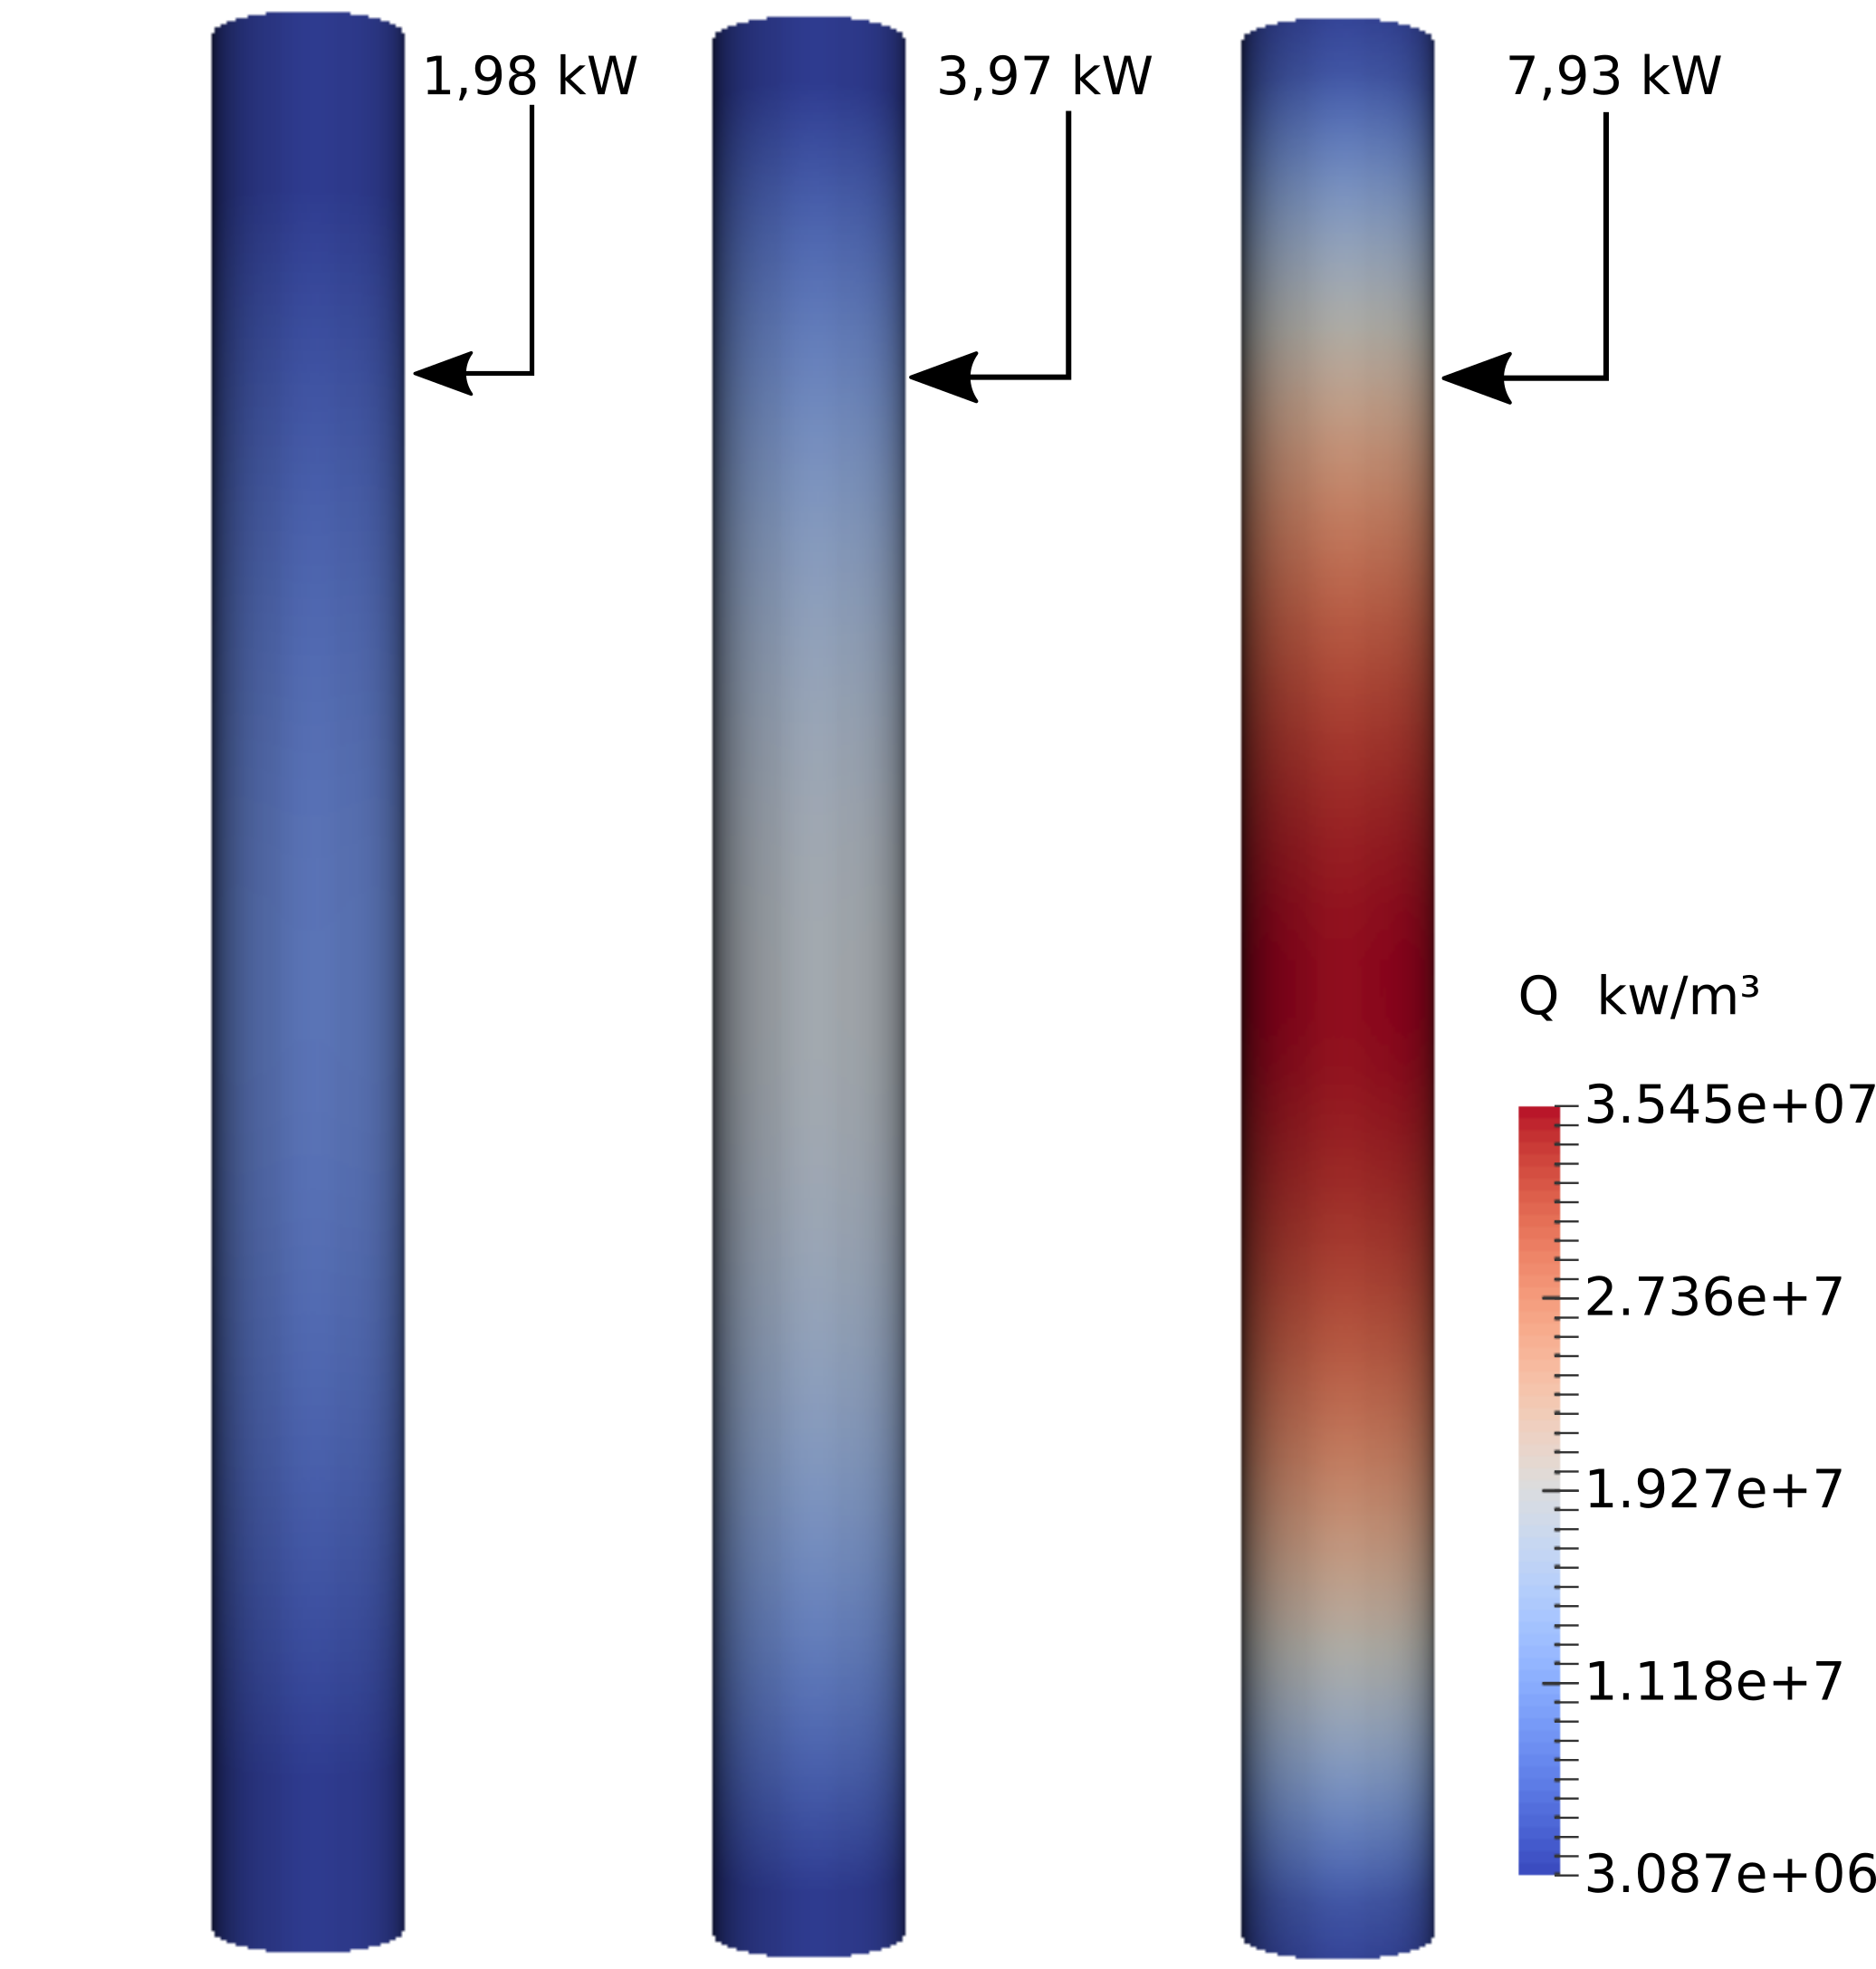
\includegraphics[scale=0.6]{figuras/Q_fuel_all_NC.png}
  \label{fig:pot-nc}
%  \legend{Fonte: autor}
\end{figure}

As distribuições de potência axial obedeceram, para os três casos, a perfis
cossenoidais, como pode ser visto na Figura \ref{fig:perf-nac-axial}. Estes são os perfis esperados para
os combustíveis modelados \cite{Veloso2005}. As distribuições de potência radiais -
obtidas do corte no ponto médio do modelo do combustível - possuem perfis diferentes \ref{fig:perf-Q-nac-radial}
dos obtidos axialmente. A primeira e principal diferença está na abruta subida a partir da potência nula
no início e fim da curva. A razão para este comportamento é simples: apenas o combustível gera potência, sendo
zero para as regiões de revestimento e água (não apresentadas na curva). O achatamento na posição central
da curva em relação aos picos é devido ao menor fluxo térmico no centro do combustível. Nas regiões limite
entre o combustível e o revestimento, é maior o fluxo de nêutrons termalizados pela interação com o refrigerante (água).
Esse perfil é esperado em combustíveis do tipo TRIGA \cite{Ravnik1990}.

\begin{figure}[htb]
  \caption{Perfil de potência axial para os três casos simulados.}
  \centering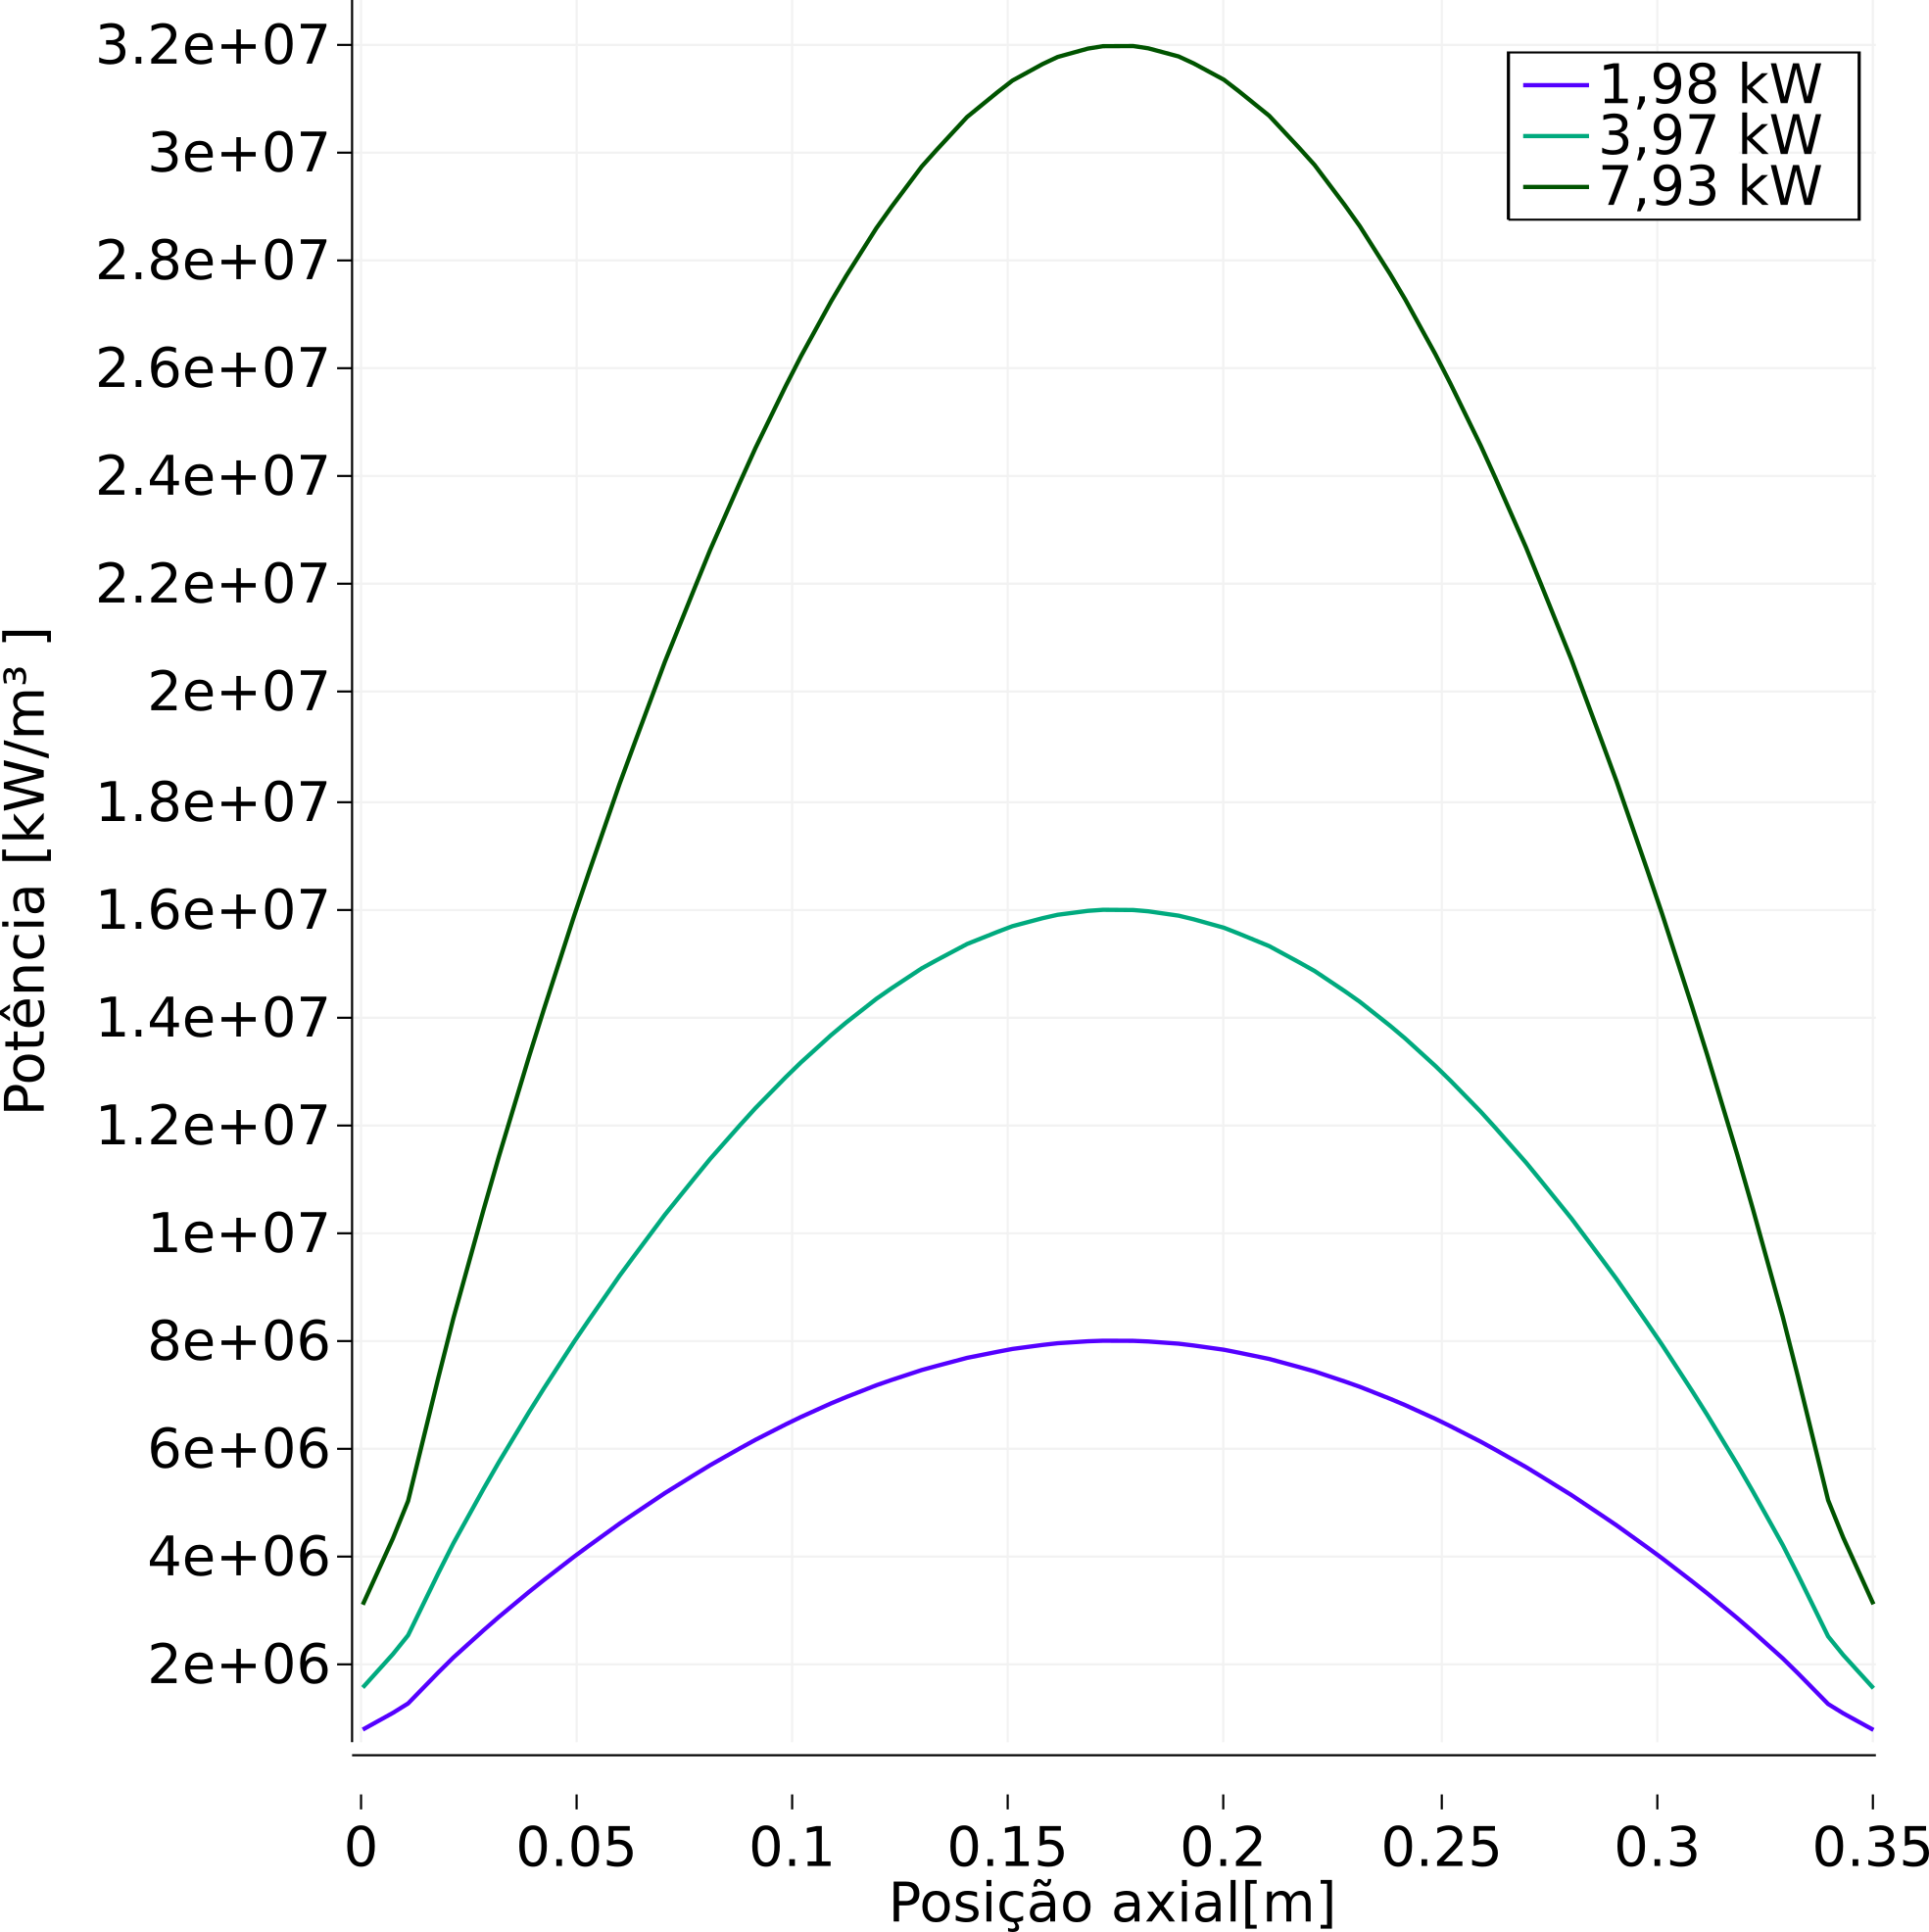
\includegraphics[scale=0.6]{figuras/Q_all_NC_port.png}
  \label{fig:perf-nac-axial}
%  \legend{Fonte: autor}
\end{figure}

\begin{figure}[htb]
  \caption[Perfil de potência radial para os três casos simulados.]{Perfil de potência radial para os três casos simulados.}
  \centering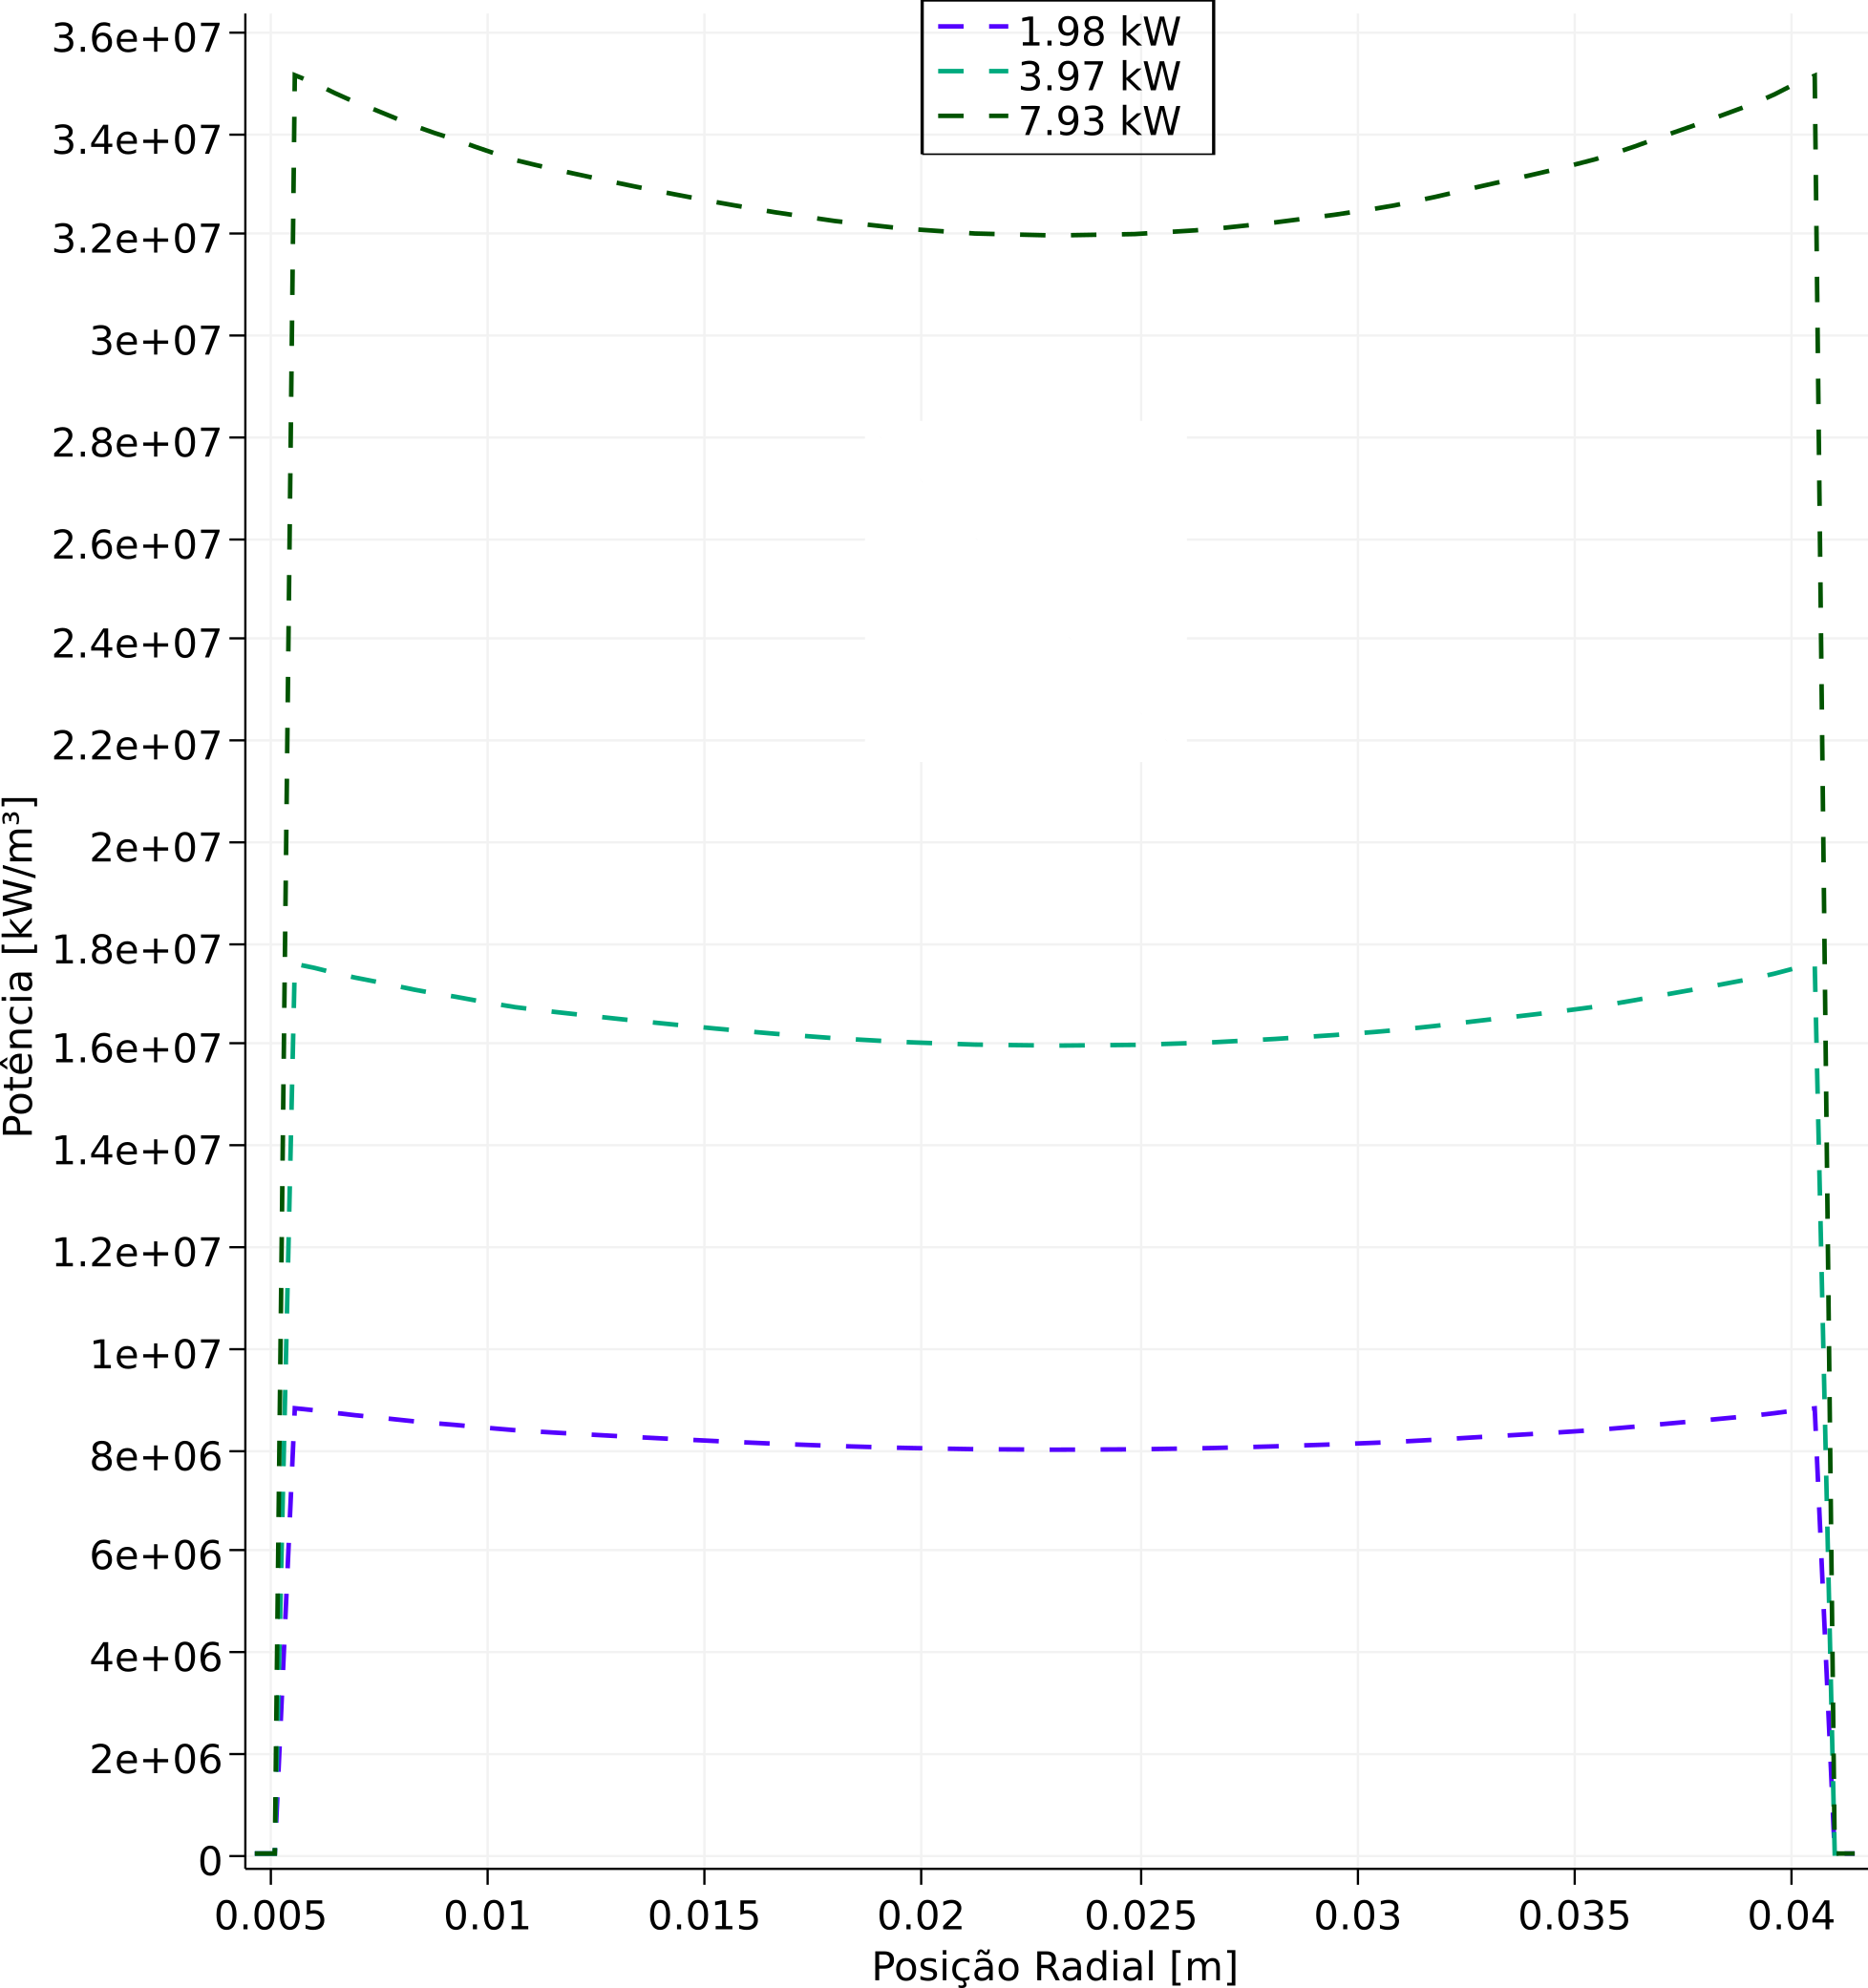
\includegraphics[scale=0.7]{figuras/Q_x_NC_square_port.png}
  \label{fig:perf-Q-nac-radial}
%  \legend{Fonte: autor}
\end{figure}

Os perfis de temperatura obtidos axialmente, Figura \ref{fig:perf-t-nac-axial},
apresentam, novamente para os três casos, uma diferença entre as extremidades
do combustível. Essa diferença é provocada pela escoamento do refrigerante (água) no
modelo. A água entra no sistema à temperatura constante de $300 K$ e, no seu trajeto,
absorve energia do sistema. Essa absorção é maior no na entrada (\textit{inlet}),
levando a uma maior resfriamento do sistema neste ponto do escoamento. Esse efeito
ocorre em todos os casos, apenas com diferença nas temperaturas de cada material.

\begin{figure}[htb]
  \caption{Perfil de temperaturas axial para os três casos simulados.}
  \centering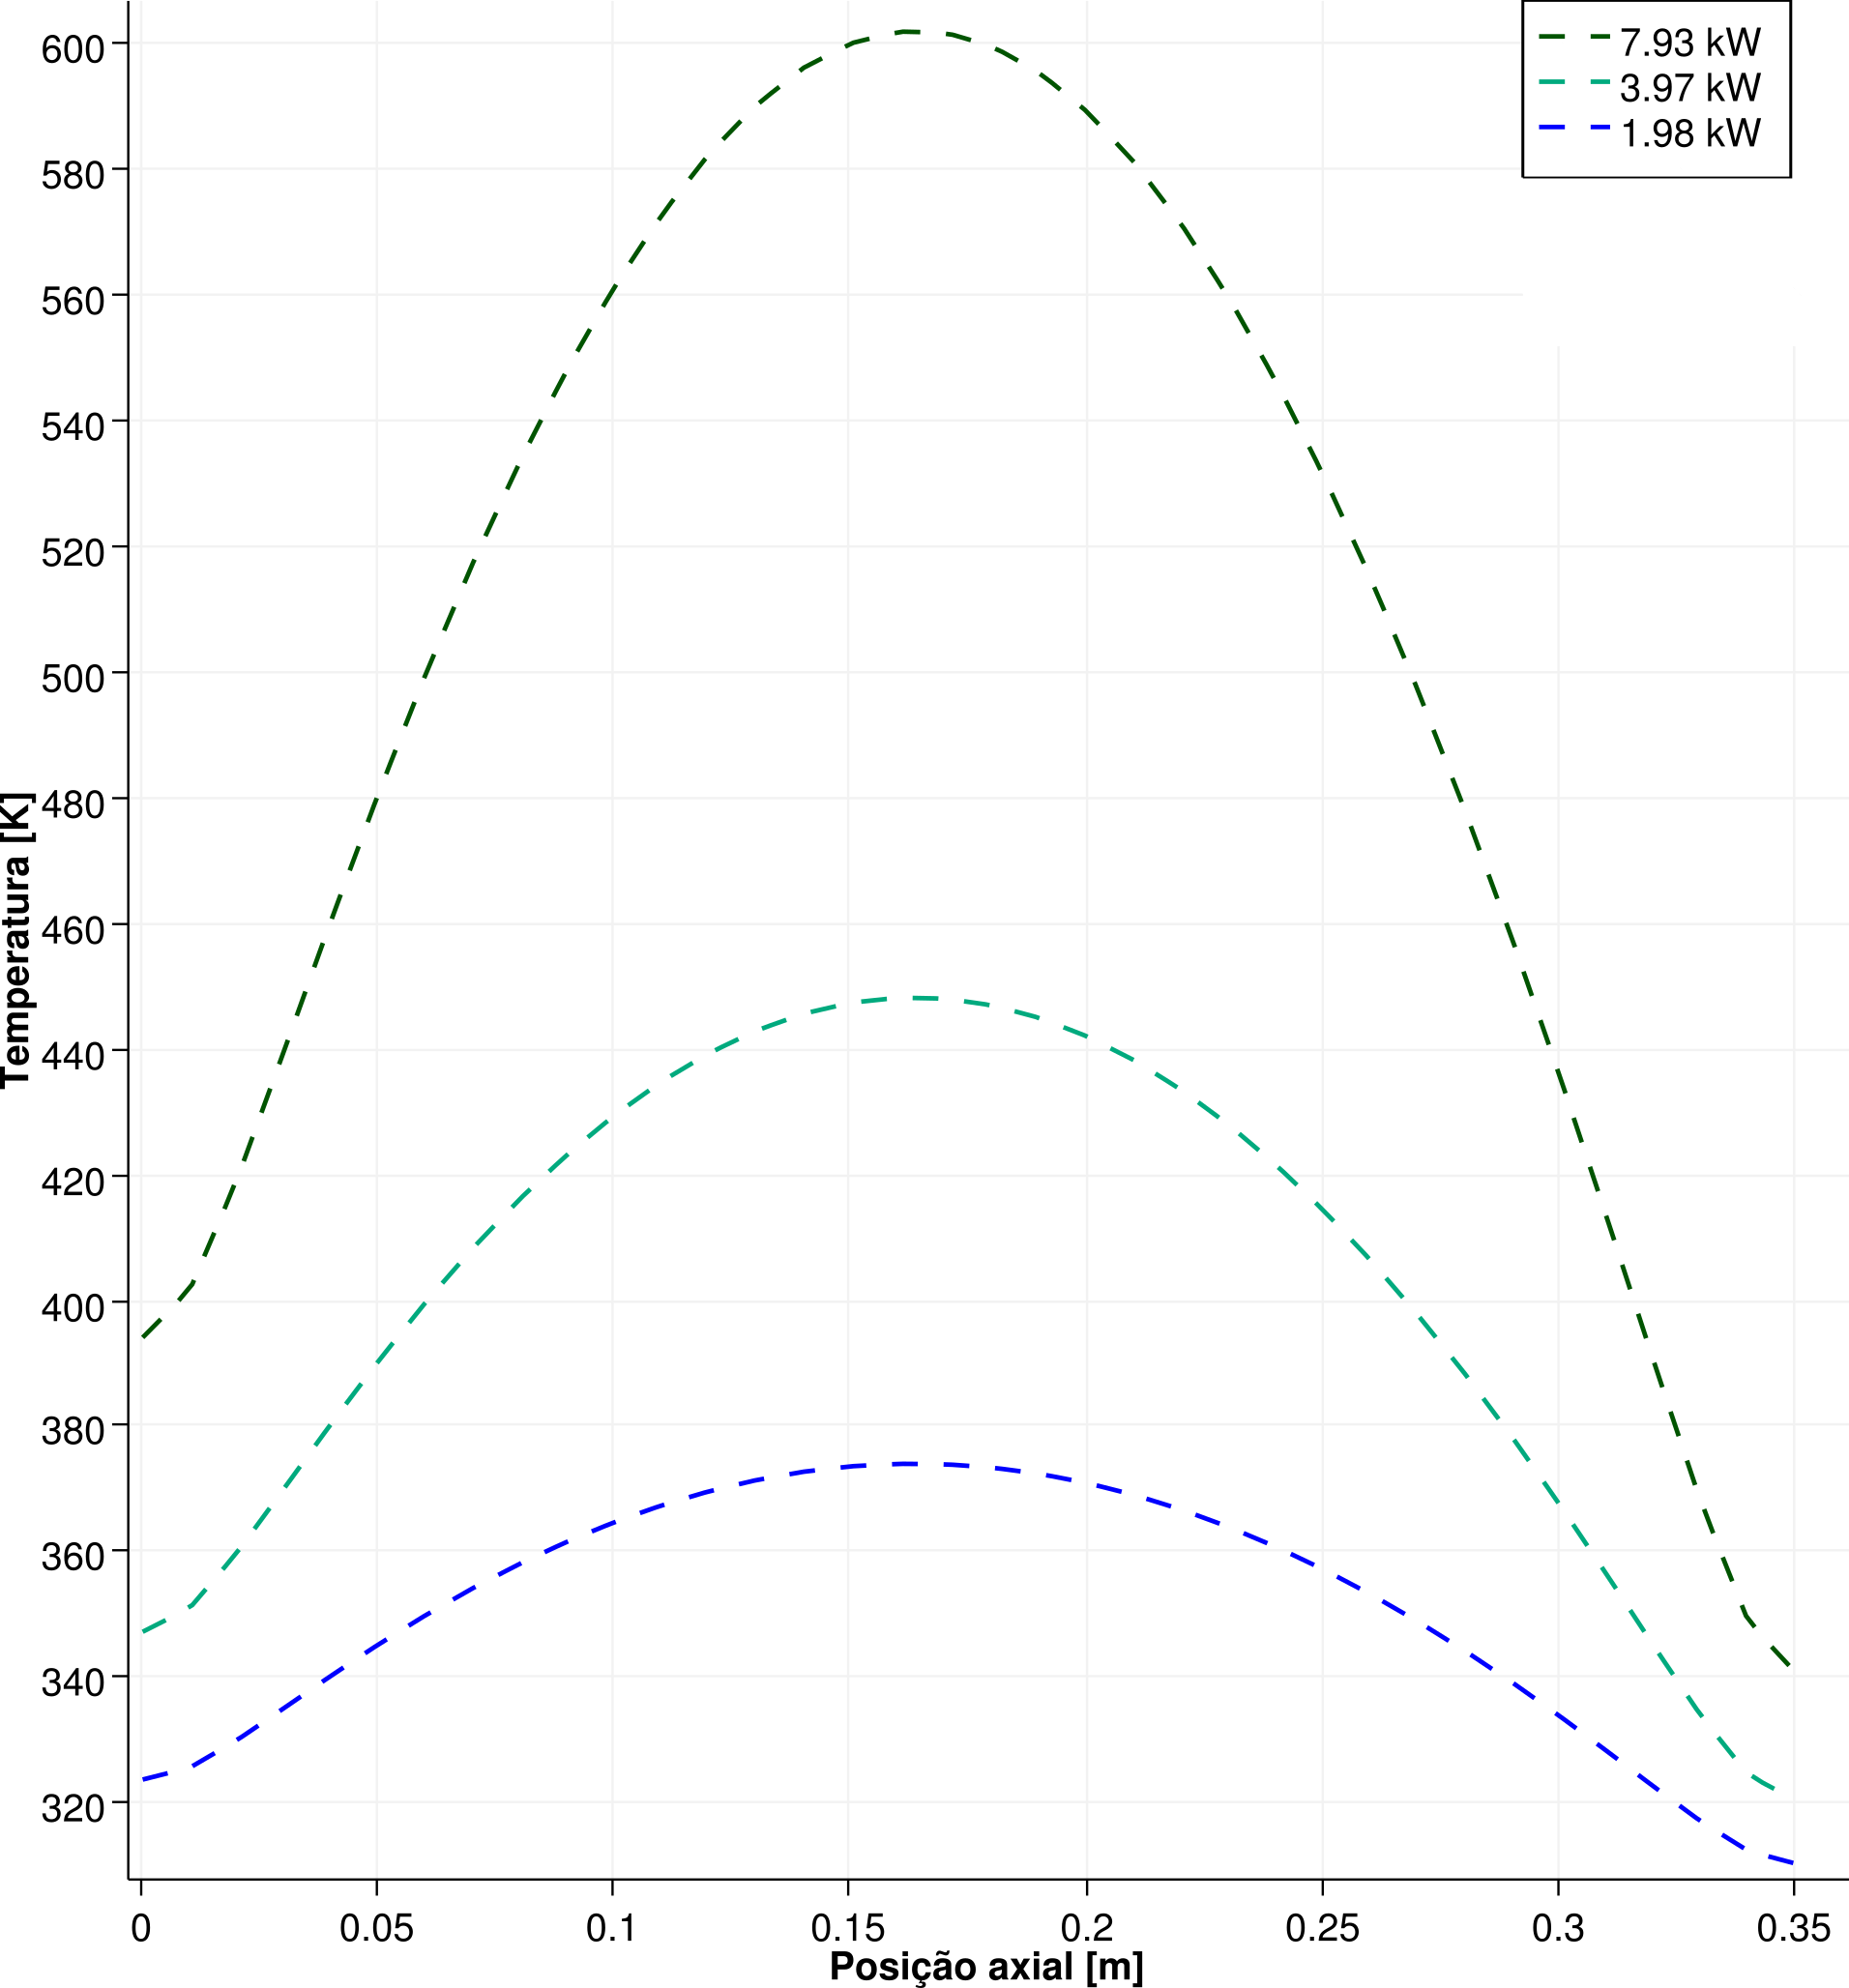
\includegraphics[scale=0.6]{figuras/T_z_NC_square_port.png}
  \label{fig:perf-t-nac-axial}
%  \legend{Fonte: autor}
\end{figure}

Radialmente, os perfis de temperatura, seguindo o mesmo padrão para os três casos simulados,
possuem descontinuidades, como pode ser visto na Figura \ref{fig:perf-t-nac-radial} (entre
$0 m$ e $0,005 m$ e $0,04 m$ e $0,045 m$). Estes degraus indicam mudança no gradiente de temperaturas na
interface entre diferentes materiais, devido às diferentes condutividades térmicas de cada um.
que ocorre no fluxo de calor entre dois materiais com propriedades físicas distintas.

Os resultados das simulações apresentadas para os três casos não-acoplados formam o conjunto de resultados
de referência. Eles servem de base de comparação para as simulações acopladas, com objetivo de verificar
se os resultados acoplados se diferenciam destes e em que medida ocorrem estas diferenças.

\begin{figure}[htb]
  \caption[Perfil de temperaturas radial para os três casos simulados.]
          {Perfil de temperaturas radial para os três casos simulados. No detalhe o perfil de temperatura nas interfaces entre os três materiais.}
  \centering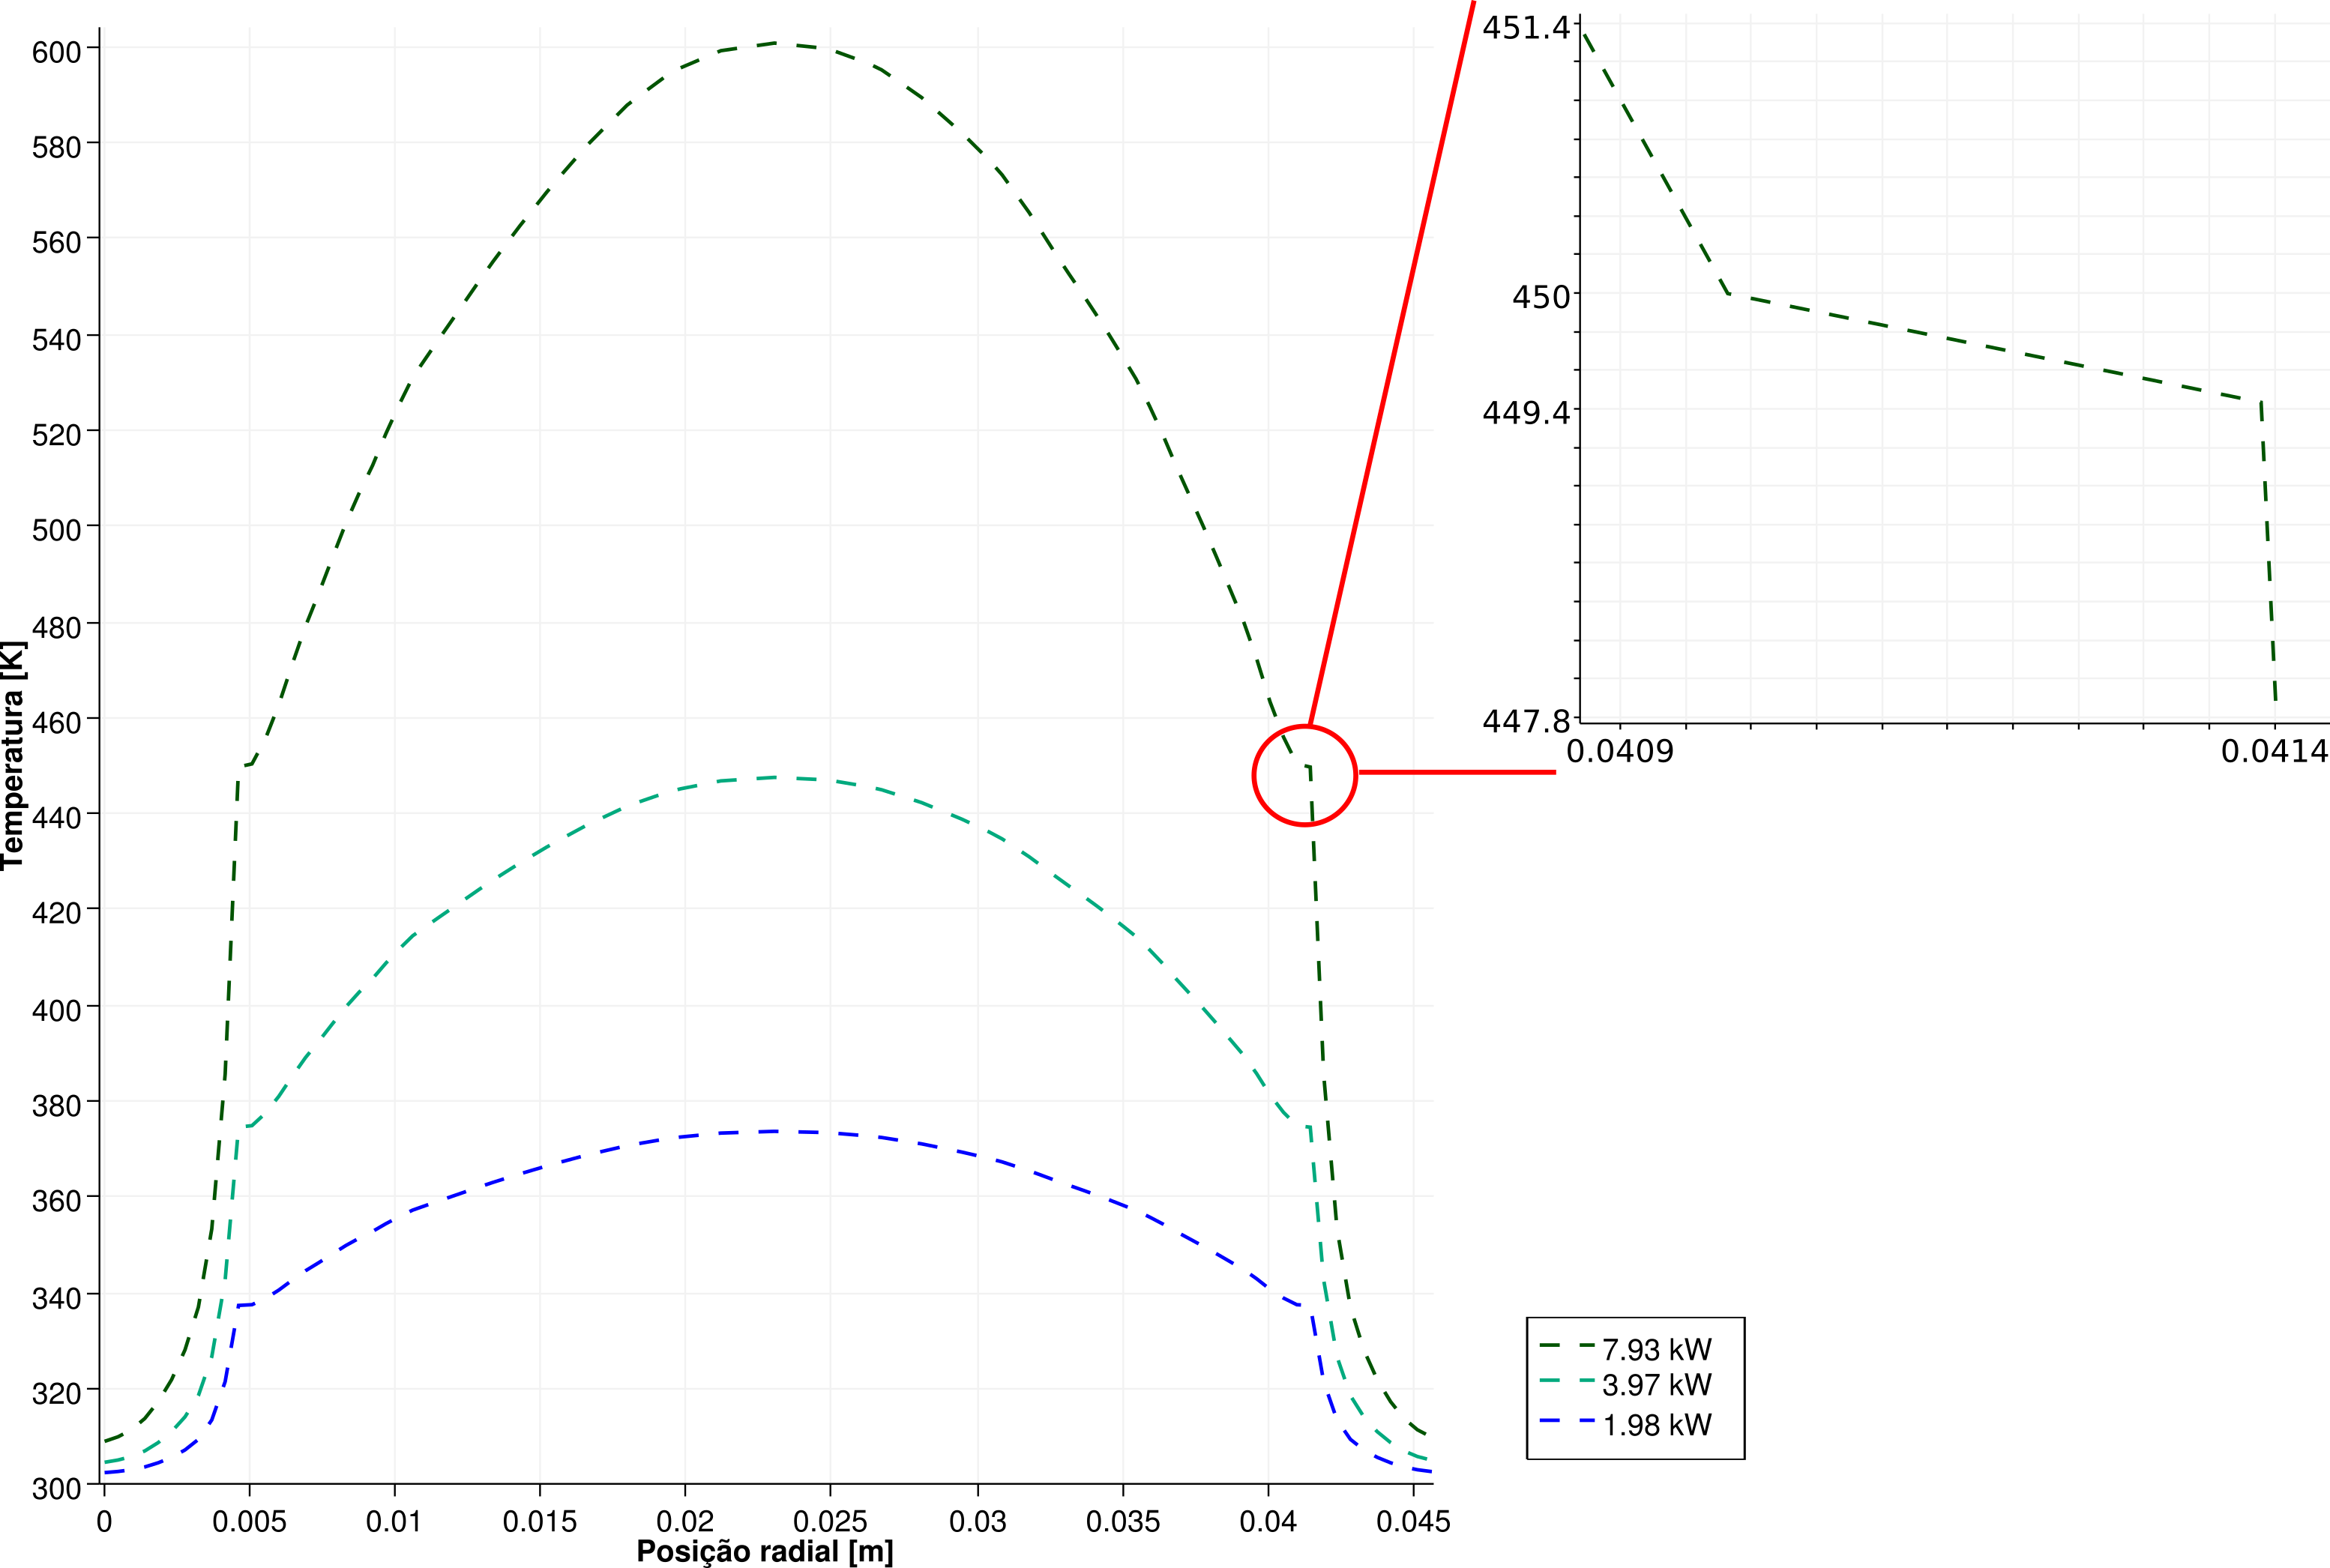
\includegraphics[scale=0.6]{figuras/T_x_NC_square_port_detalhado.png}
  \label{fig:perf-t-nac-radial}
%  \legend{Fonte: autor}
\end{figure}


% ------------------------------------------------------------------------------------------------------------
\section{Caso acoplado}
\label{sec:cp}

As simulações acopladas foram realizadas exatamente nas mesmas condições das suas homólogas não-acopladas.
Os resultados destas são apresentados em comparação com os resultados anteriores para visualização
das diferenças entre elas.

Diferentemente dos cálculos não-acoplados, na simulação acoplada ocorre a variação do fluxo neutrônico.
Essa variação, originada da variação de temperaturas no sistema, ocorre nos três casos acoplados, cada
um simulado numa potência.

Para as simulações a $1,98 kW$, as diferenças no fluxo são as mais sutis. Com potência mais baixa, há menor
diferença nas temperaturas entre o caso acoplado e o não-acoplado. Como as seções de choque variam de
acordo com a temperatura, é menor a diferença entre seções de choque. Por consequência, menor a diferença
no fluxo neutrônico. Outro fator que leva à similaridade entre os fluxos é a baixa granularidade
da malha na direção axial (apenas 35 camadas de elementos, como apresentado na Tabela \ref{tab:size_model}).

Na Figura \ref{fig:flux_z_50} são apresentados os fluxos axiais acoplados e não acoplados nas simulações
à potência mais baixa, de $1,98 kW$. A diferença entre os fluxos é melhor percebida no corte radial,
apresentado na Figura \ref{fig:flux_x_50}. Além de uma maior variação radial devido à moderação de nêutrons
nas paredes, e consequente aumento do fluxo térmico, a malha é radialmente mais refinada. Com isso, é possível
captar mais detalhes do fluxo neutrônico.

%Ver se dá pra colocar tempo e parâmetros de convergência.

\begin{figure}[htb]
  \caption{Fluxos relativos axiais entre simulação acoplada e não acoplada para
    potência de 1,98 kW.}
  \centering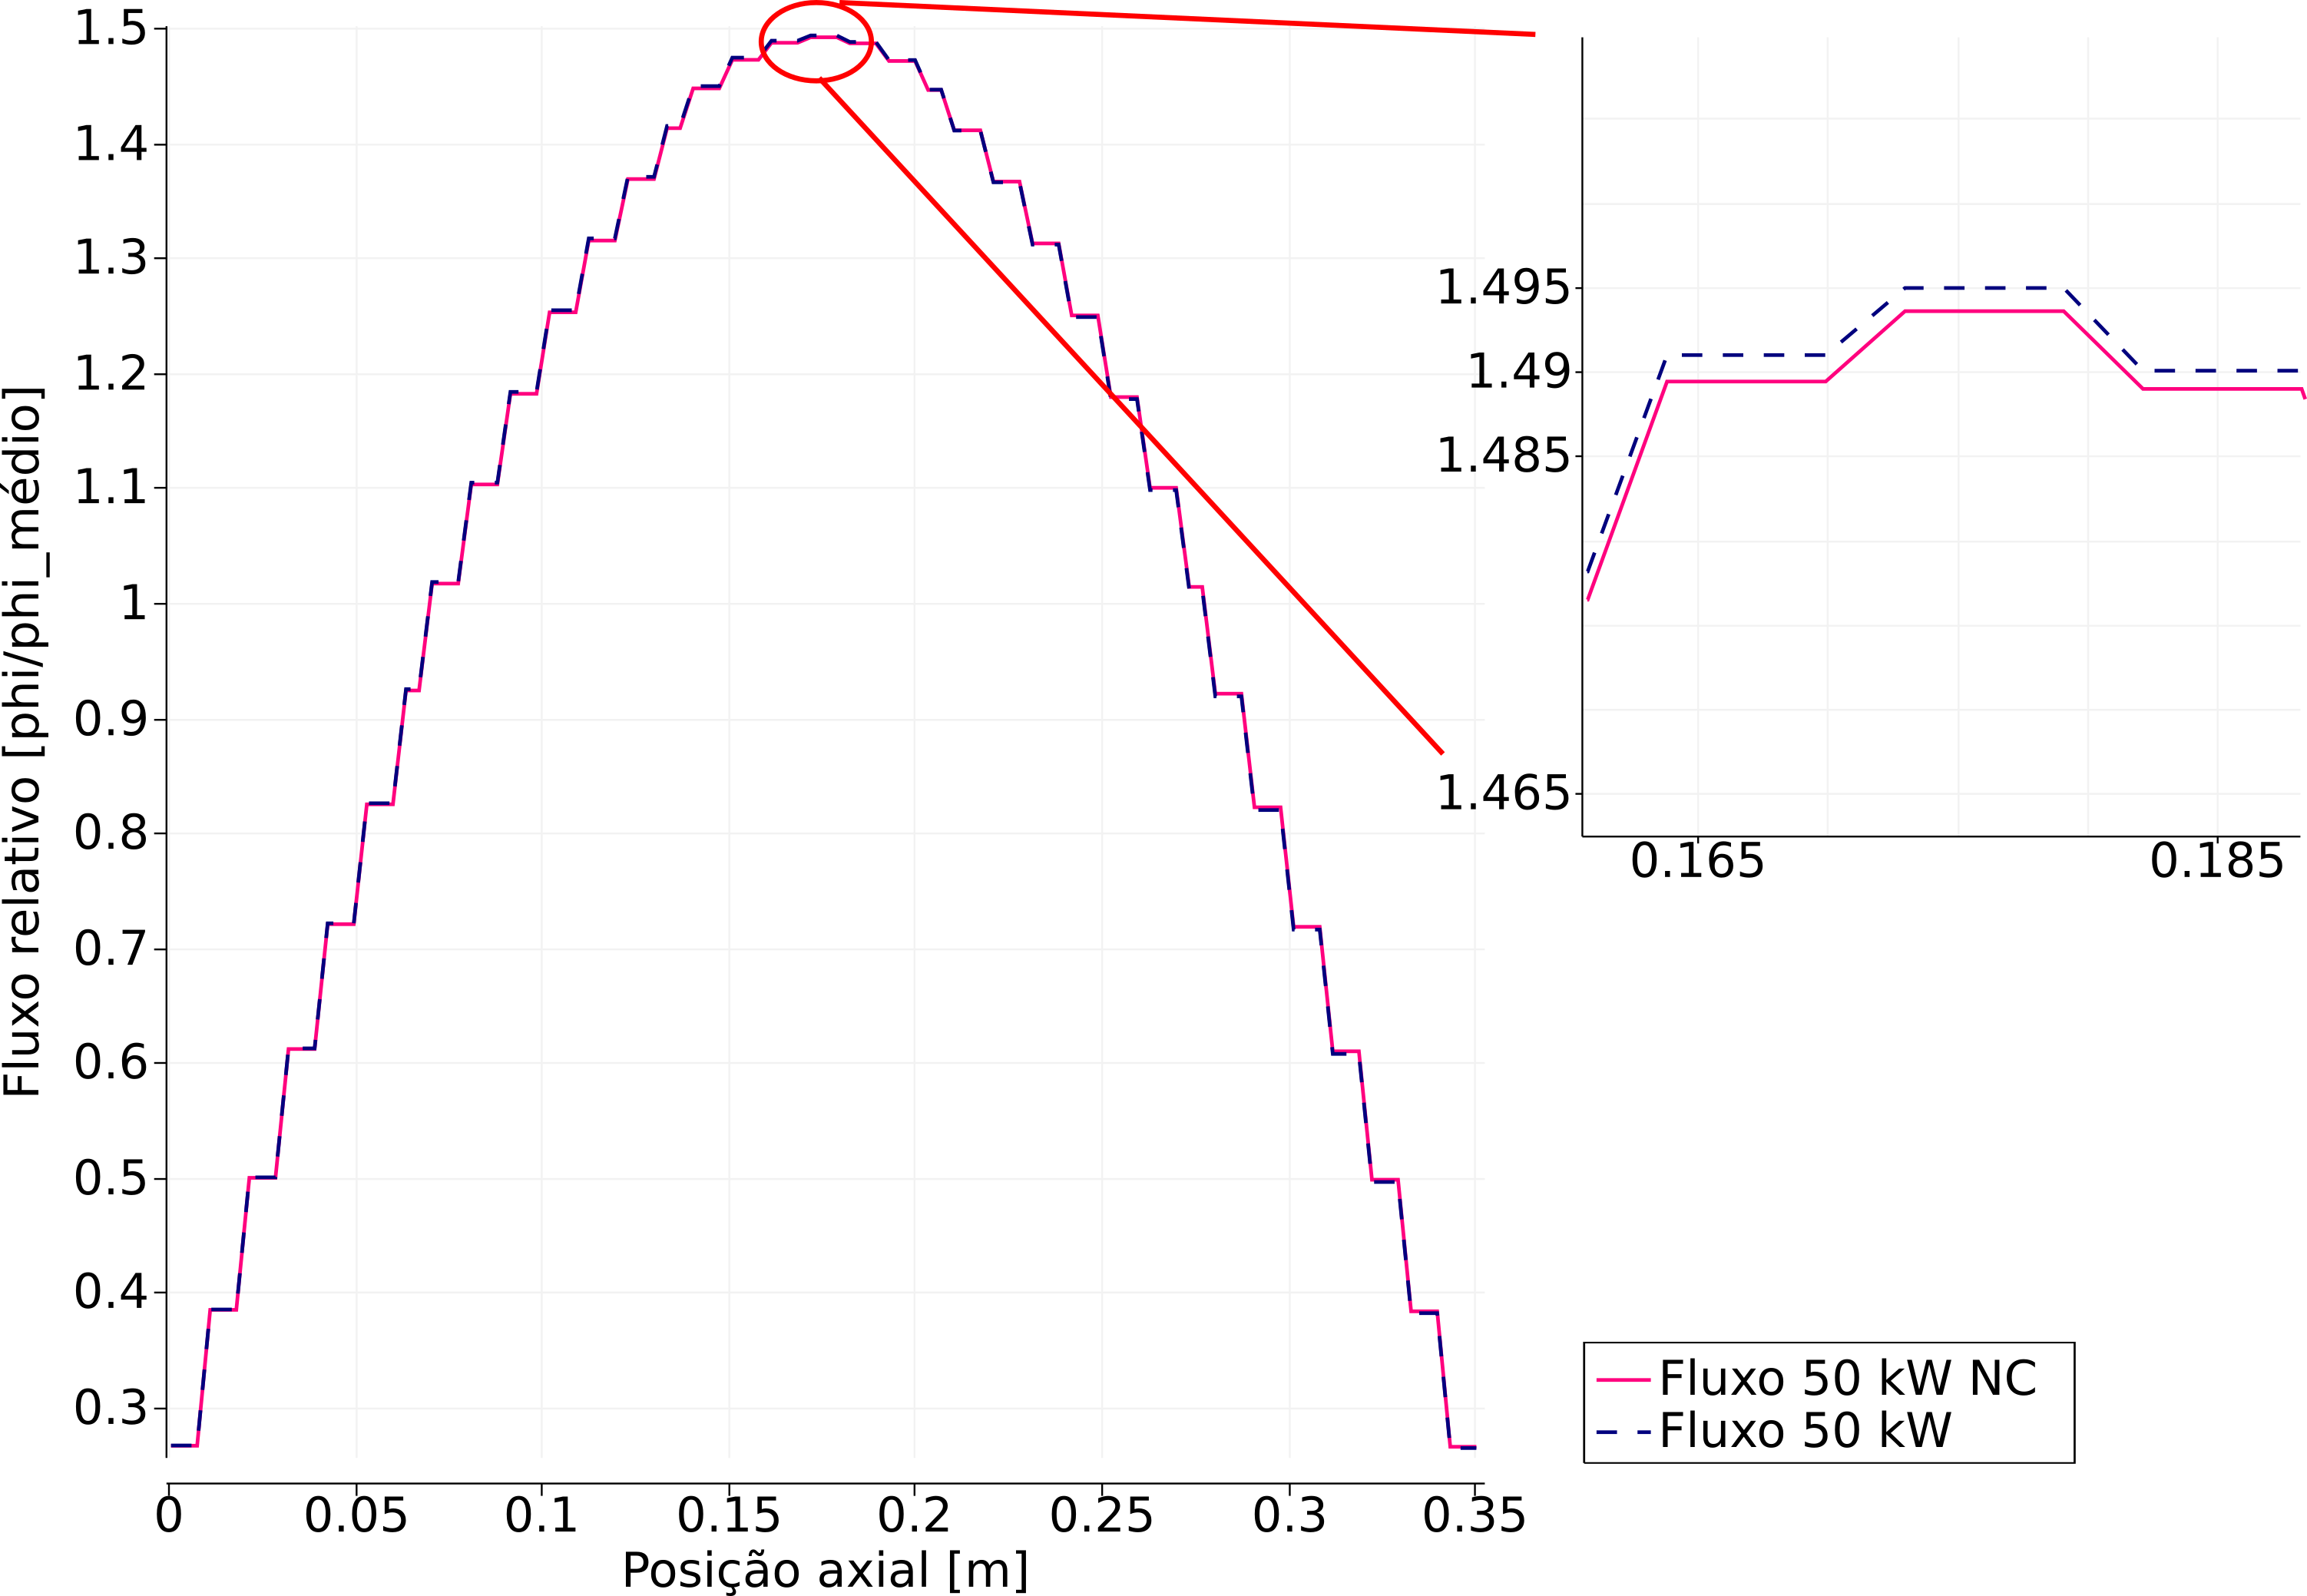
\includegraphics[scale=0.6]{figuras/Flux_rel_z_50_port_trabalhado.png}
  \label{fig:flux_z_50}
%  \legend{Fonte: autor}
\end{figure}

\begin{figure}[htb]
  \caption{Fluxos relativos radiais entre simulação acoplada e não acoplada para
    potência de 1,98 kW.}
  \centering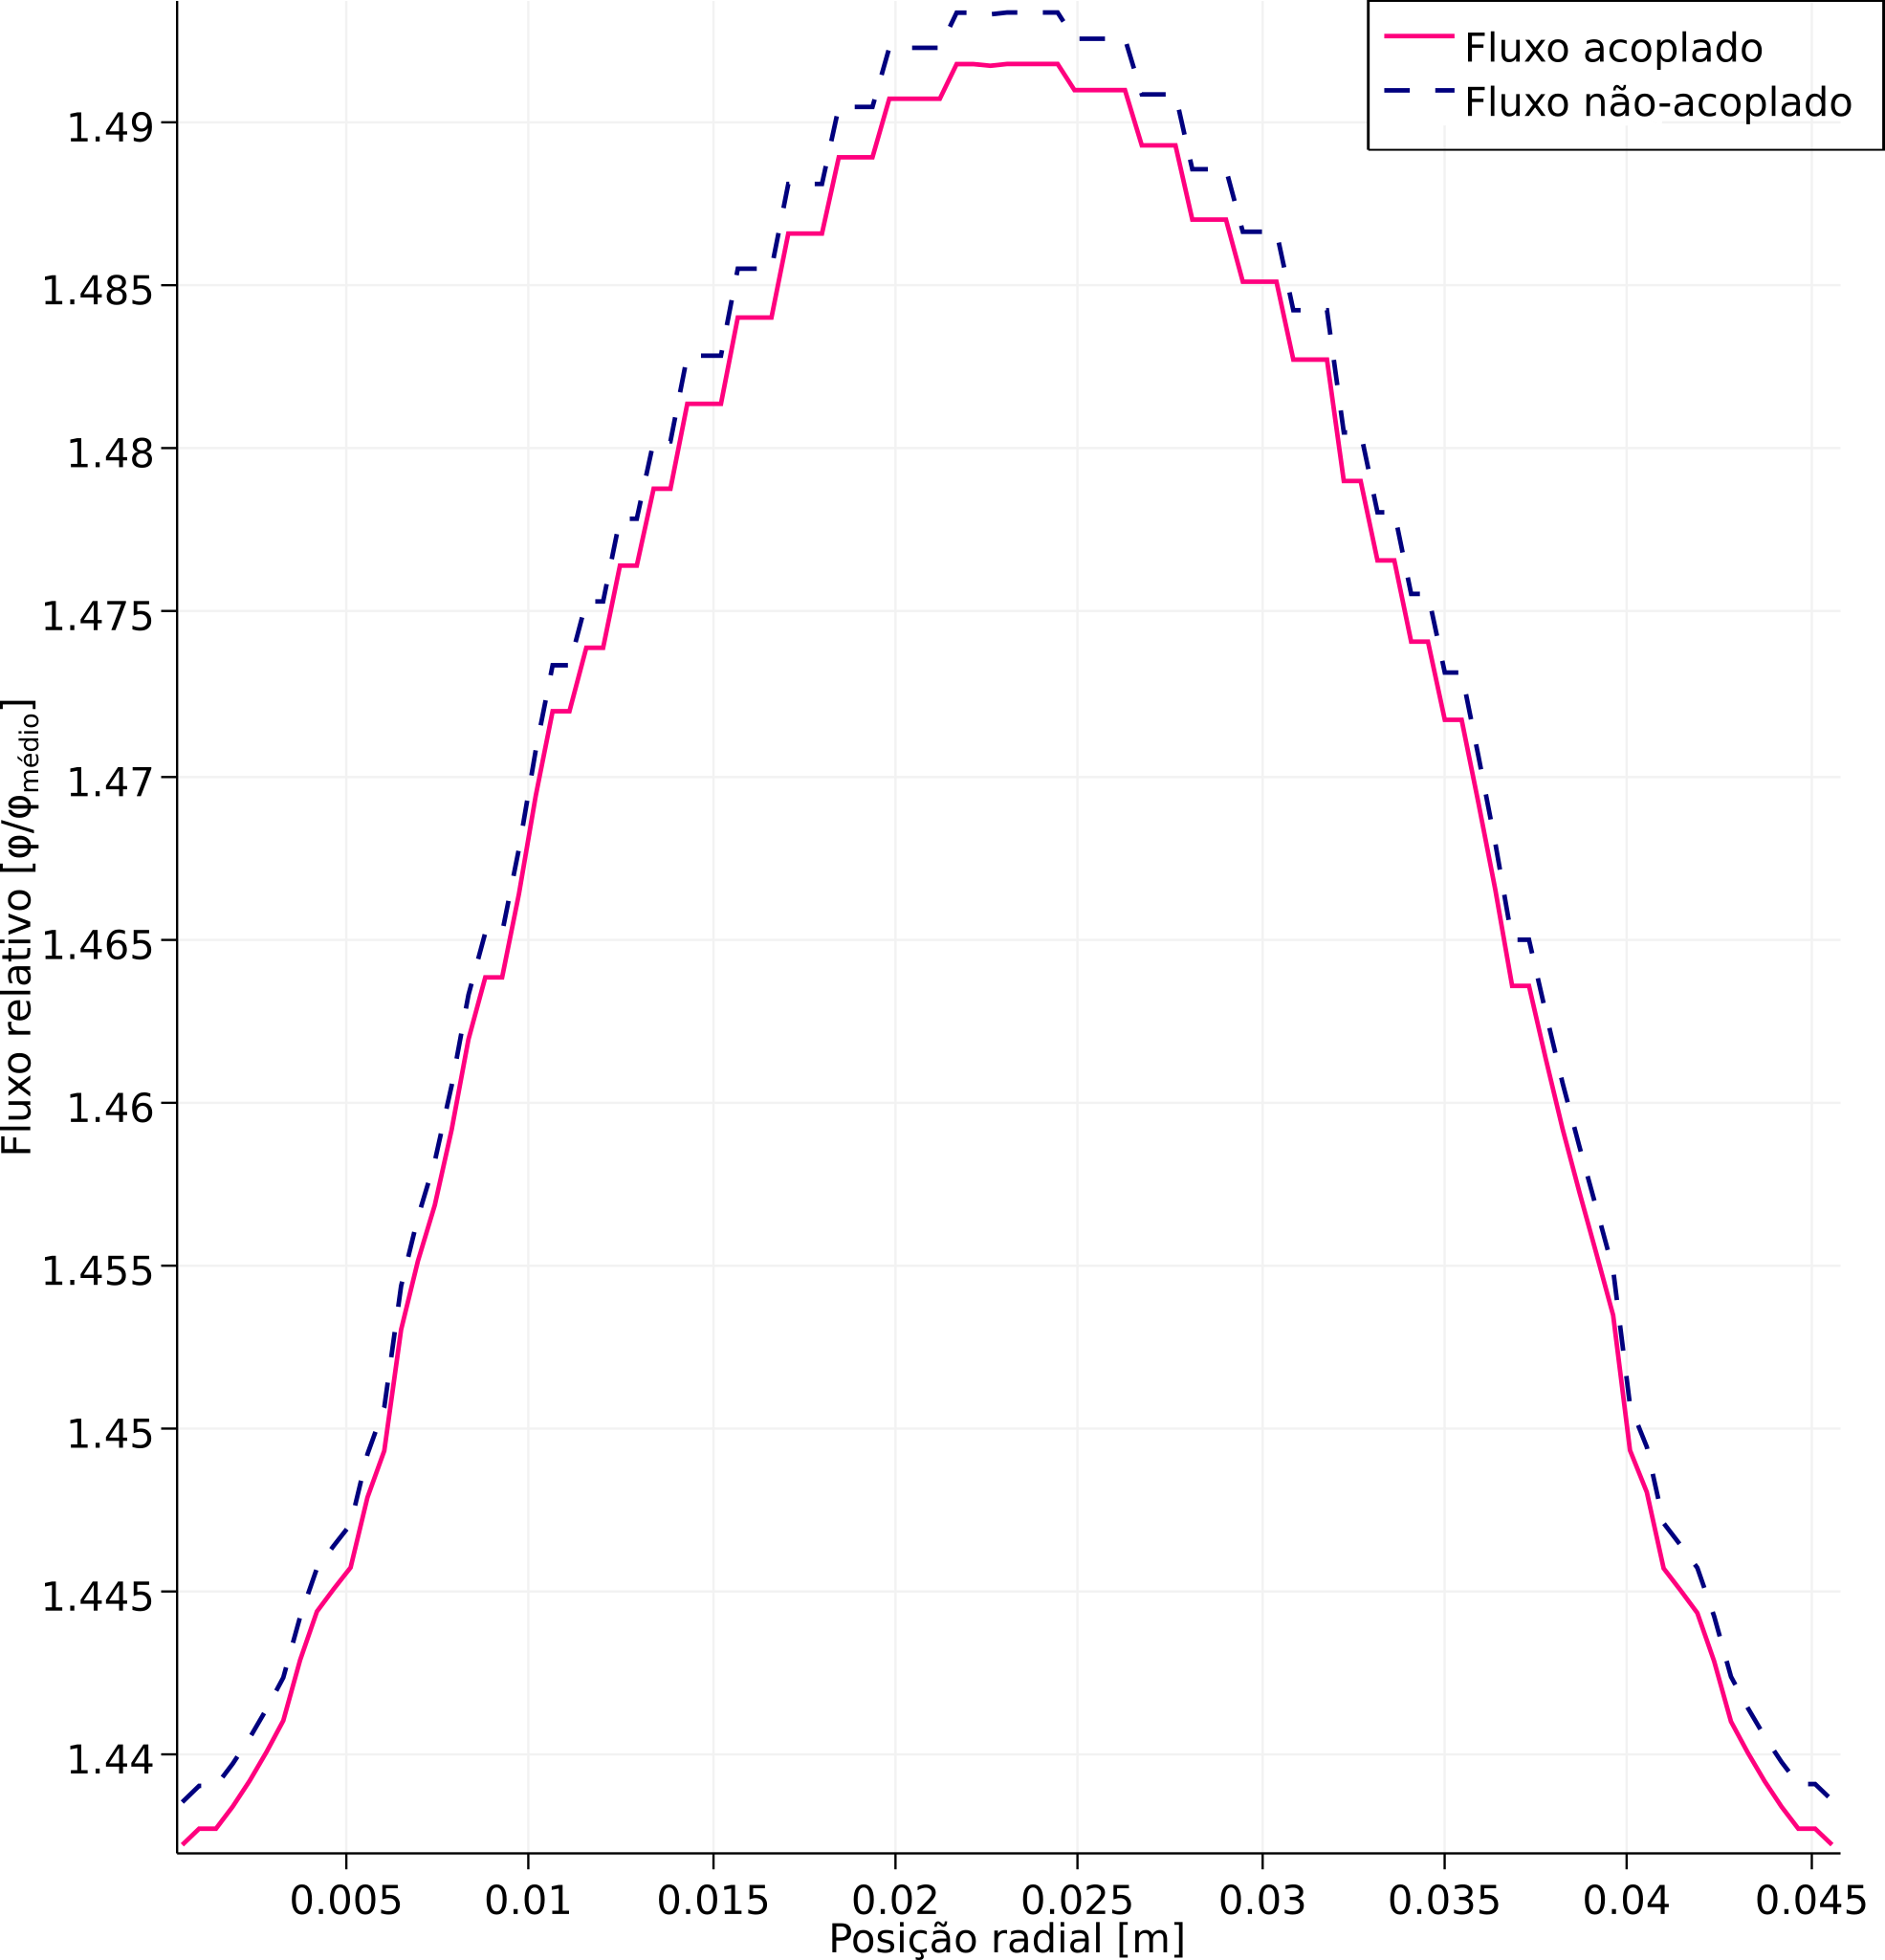
\includegraphics[scale=0.7]{figuras/Flux_rel_x_50_port.png}
  \label{fig:flux_x_50}
%  \legend{Fonte: autor}
\end{figure}

As mesmas observações feitas para os fluxos relativos na menor potência são válidas
para as simulações feitas à potência de $3,97 kW$. Novamente, as diferenças entre
os fluxos relativos são melhor observáveis no corte radial do que no corte axial.
Entretanto, as diferenças entre os fluxo começam a aumentar de acordo com o
aumento da potência. Os fluxos relativos axiais acoplados e não-acoplados para
potência de $3,97 kW$ podem ser observados na Figura \ref{fig:flux_z_100}, enquanto
os fluxos relativos radiais para a mesma potência podem ser observados na Figura \ref{fig:flux_x_100}.

\begin{figure}[htb]
  \caption{Fluxos relativos axiais entre simulação acoplada e não acoplada para
    potência de 3,97 kW.}
  \centering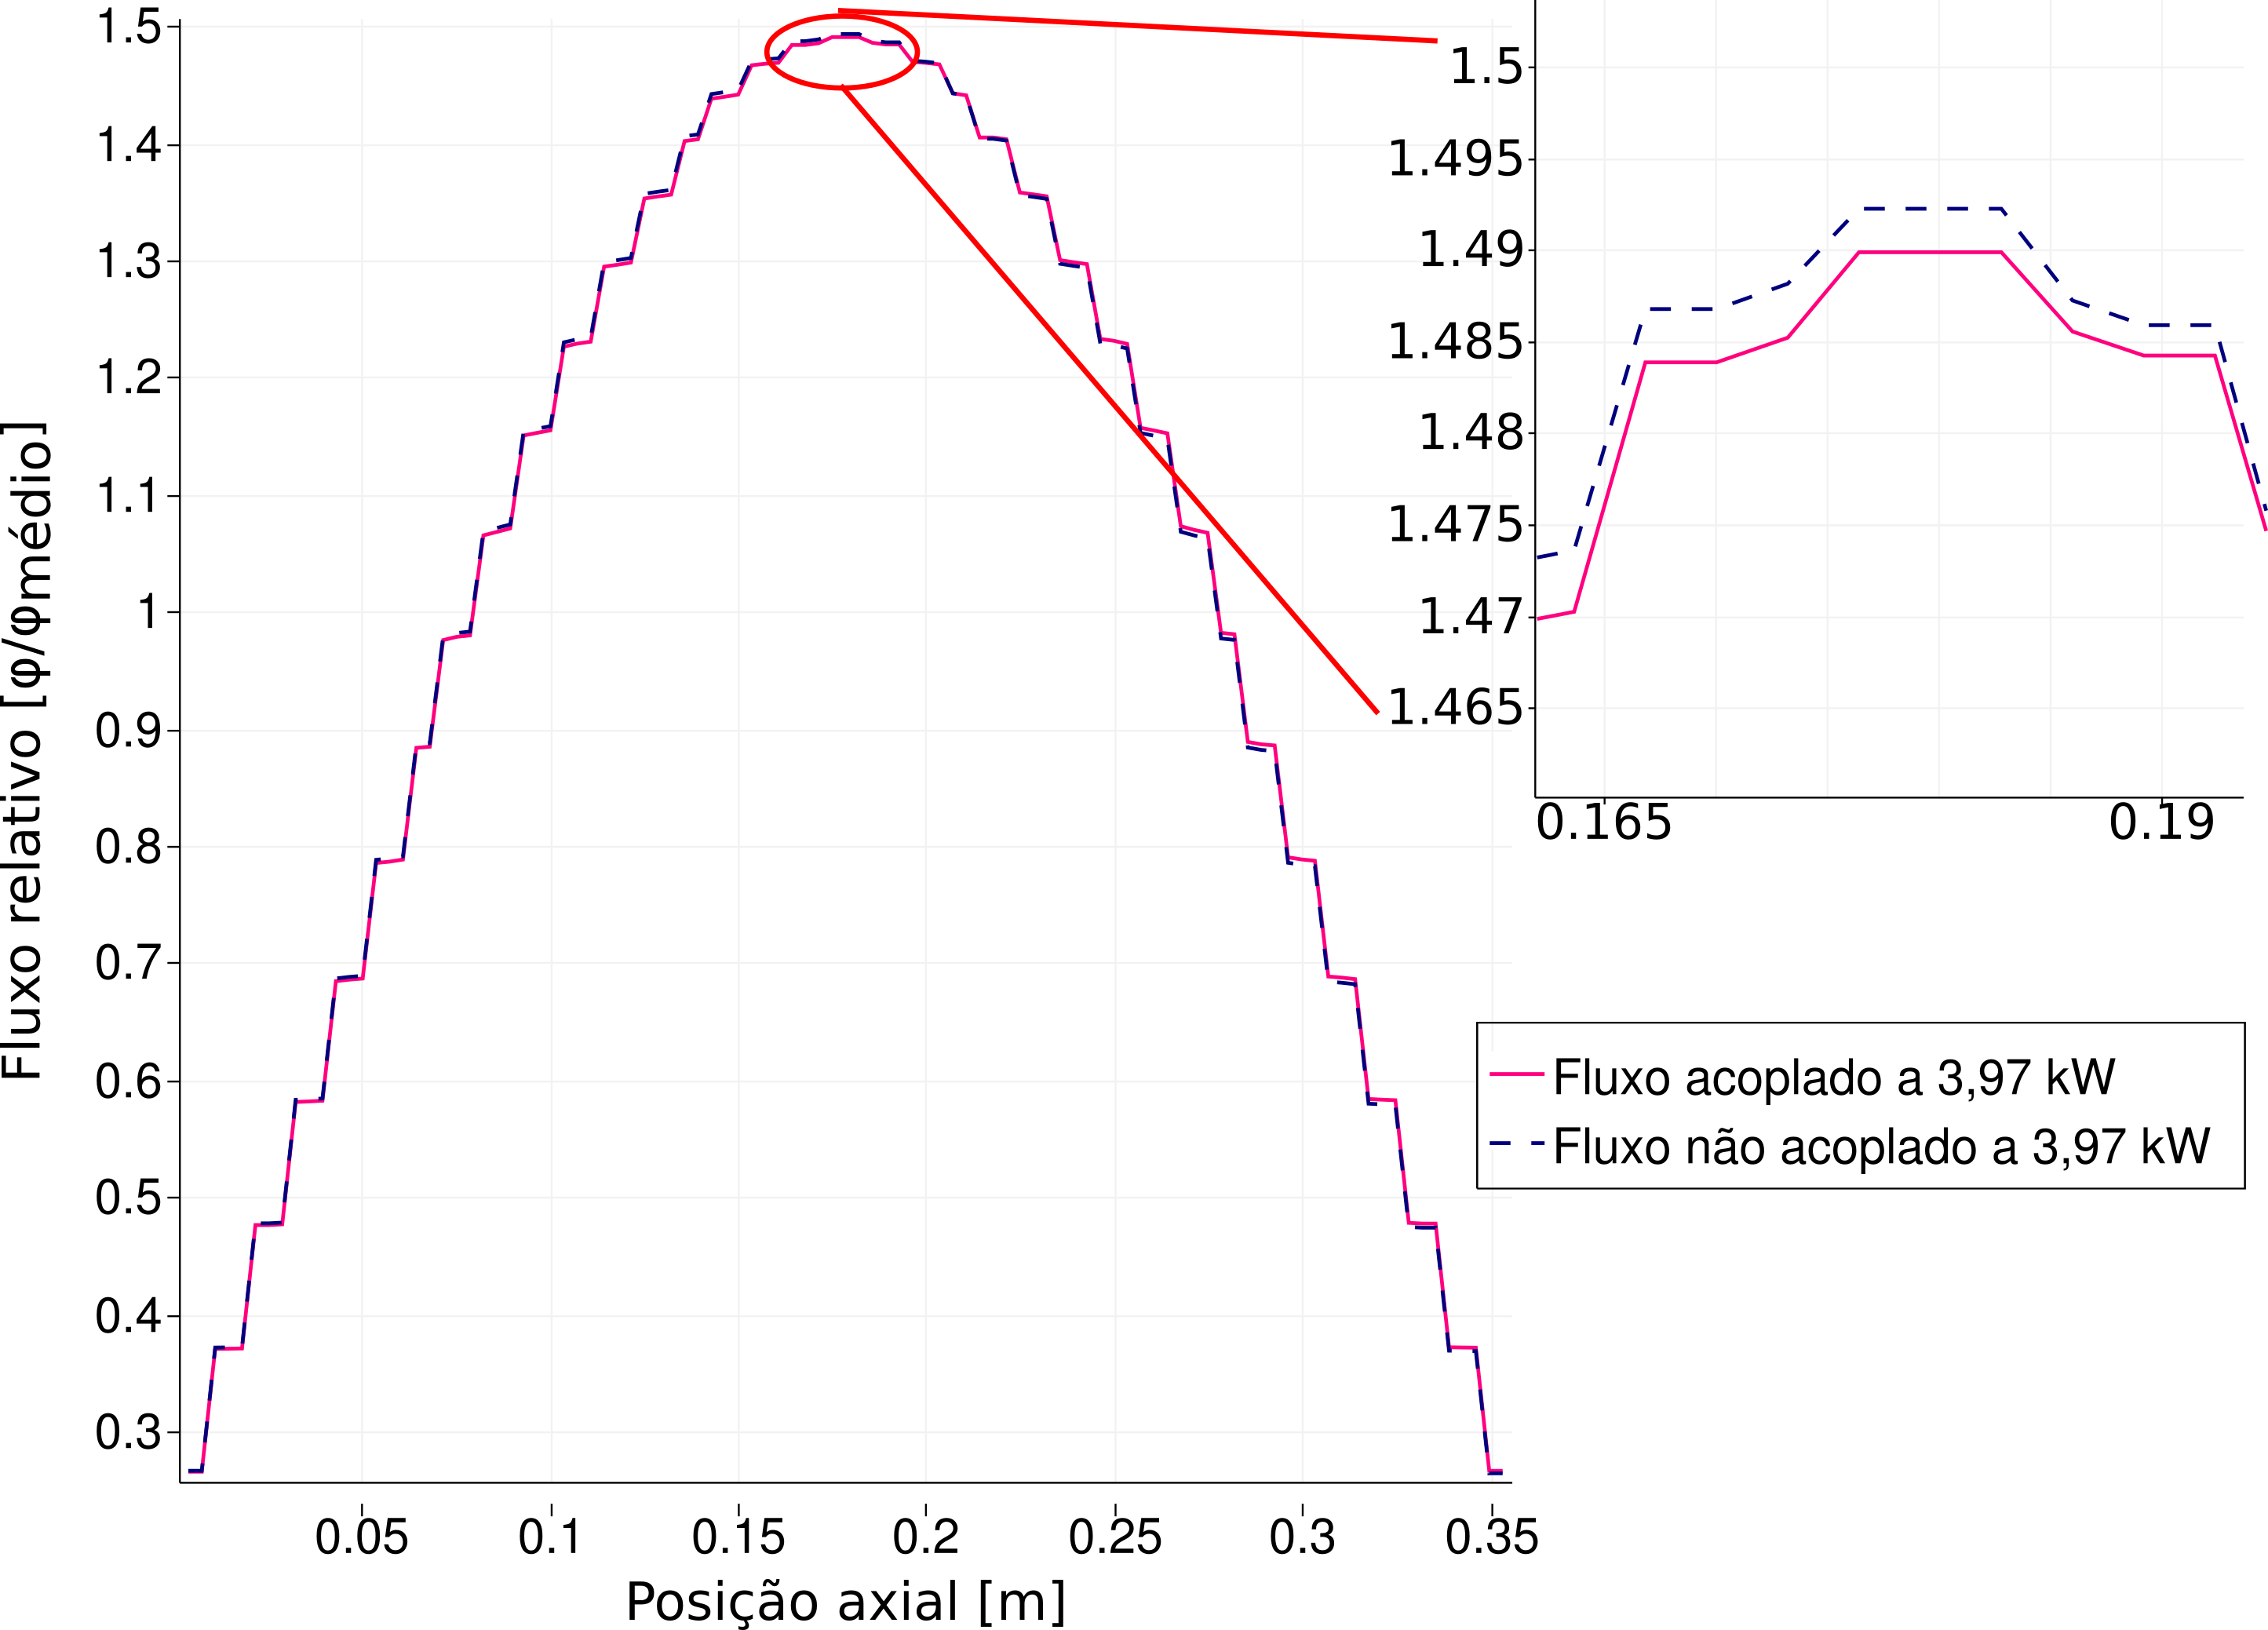
\includegraphics[scale=0.6]{figuras/Flux_rel_z_100_port_trabalhado.png}
  \label{fig:flux_z_100}
%  \legend{Fonte: autor}
\end{figure}

\begin{figure}[htb]
  \caption{Fluxos relativos radiais entre simulação acoplada e não acoplada para
    potência de 3,97 kW.}
  \centering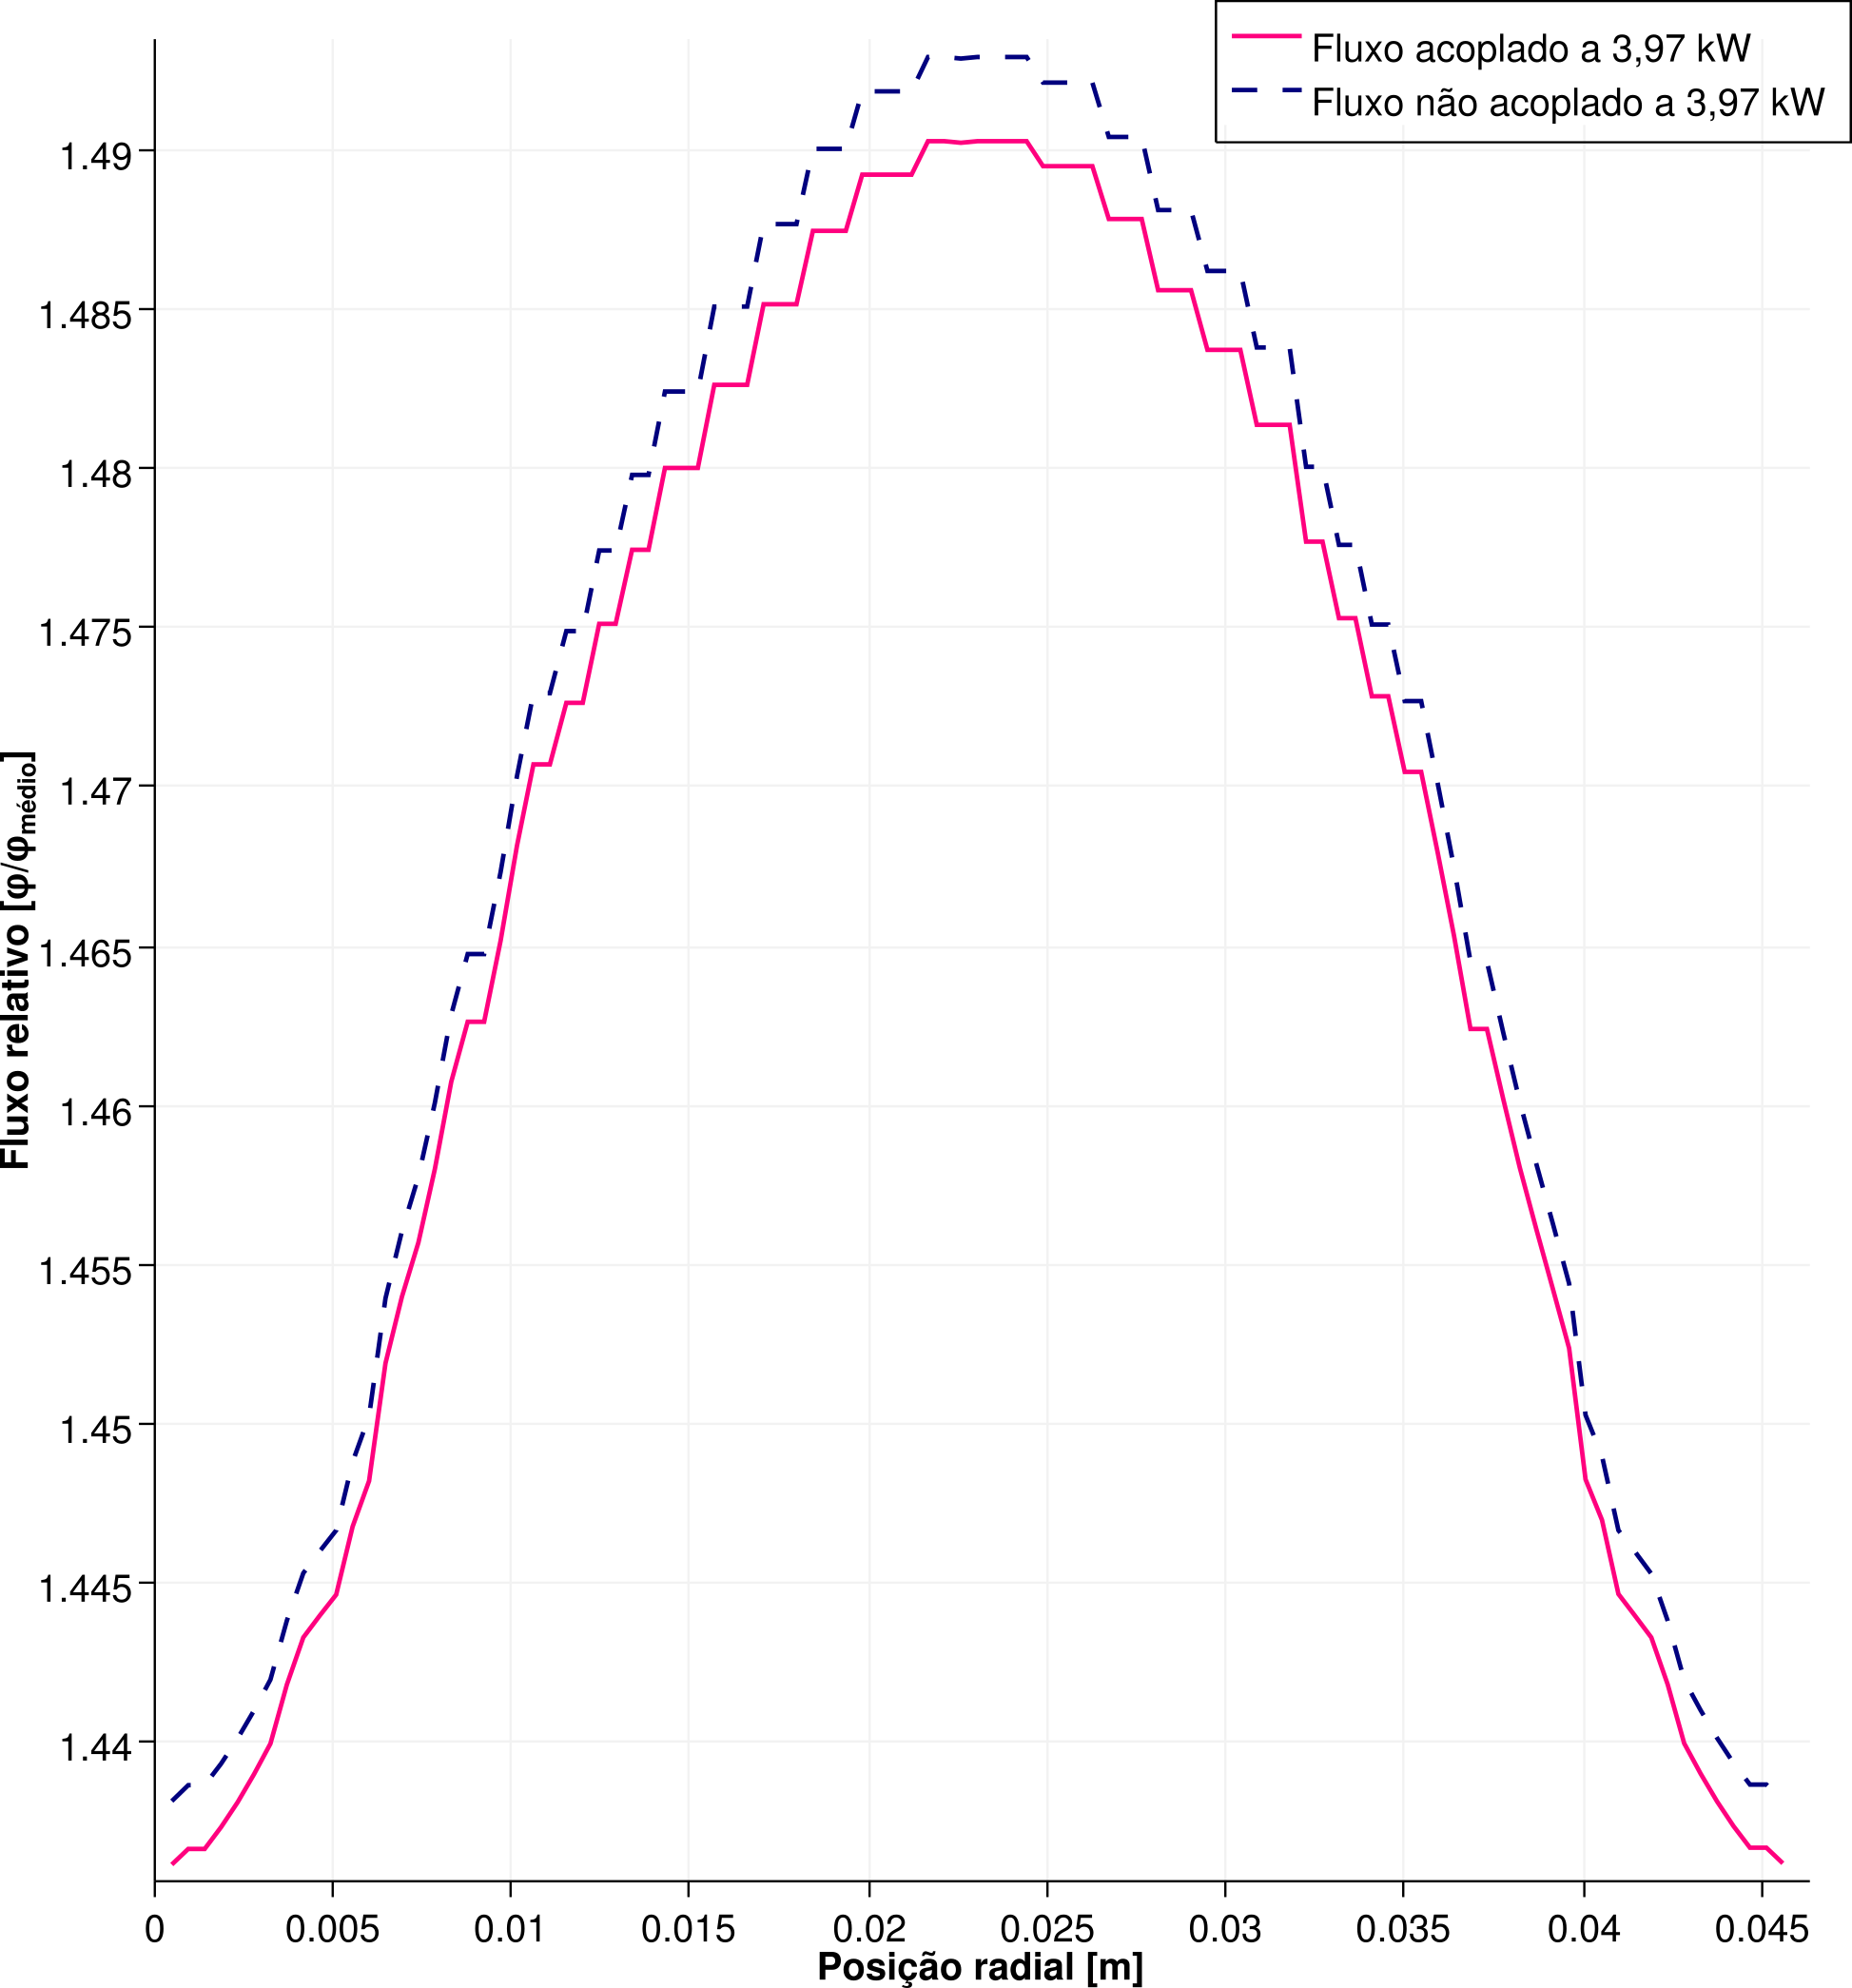
\includegraphics[scale=0.7]{figuras/Flux_rel_x_100_port.png}
  \label{fig:flux_x_100}
%  \legend{Fonte: autor}
\end{figure}
